\documentclass[usetitle=true, journal=jpclcd, manuscript=letter]{achemso}

\usepackage[version=4]{mhchem}
\usepackage{color}
\usepackage{geometry}
\geometry{letterpaper}                     % ... or a4paper or a5paper or ... 
%\geometry{landscape}                		   % Activate for for rotated page geometry
%\usepackage[parfill]{parskip}    		     % Activate to begin paragraphs with an empty line rather than an indent
\usepackage{graphicx}
\usepackage{subcaption}				
\usepackage{amssymb}
\usepackage{amsmath}
\usepackage{setspace}
\usepackage[T1]{fontenc}
\usepackage{siunitx} %BRJ added. is this OK??
\usepackage{chemmacros}
%\usepackage{multirow} %BRJ added
\usepackage{xspace}

\DeclareSIUnit{\molar}{M}
\DeclareSIUnit[number-unit-product = {\,}]
\cal{cal}
\DeclareSIUnit\kcal{\kilo\cal}


\newcommand{\kon}{$k_{\textrm{on}}$\xspace}
\newcommand{\koff}{$k_{\textrm{off}}$\xspace}
\let\oldAA\AA
\renewcommand{\AA}{\oldAA\xspace}
\newcommand{\bcd}{$\beta$-cyclodextrin\xspace}


\title{Supporting Information: Quantitative Ranking of Ligand Binding Kinetics with a Multiscale Milestoning Simulation Approach}

% author list
\author{Benjamin R. Jagger} 
\affiliation[Dept. of Chemistry and Biochemistry, University of California, San Diego]
{Department of Chemistry and Biochemistry, University of California, San Diego, 
9500 Gilman Drive, La Jolla, California 92093-0340, United States}

\author{Christopher T. Lee} 
\affiliation[Dept. of Chemistry and Biochemistry, University of California, San Diego]
{Department of Chemistry and Biochemistry, University of California, San Diego, 
9500 Gilman Drive, La Jolla, California 92093-0340, United States}

\author{Rommie E. Amaro} 
\affiliation[Dept. of Chemistry and Biochemistry, University of California, San Diego]
{Department of Chemistry and Biochemistry, University of California, San Diego, 
9500 Gilman Drive, La Jolla, California 92093-0340, United States}
\email{ramaro@ucsd.edu}

\begin{document}

\newpage

%!TEX root = bcd_SI.tex

\section*{Methods}
\subsection*{System Preparation} 
\par GAFF\cite{Wang2004,Wang2006} forcefield parameters for the seven guest molecule
along with both GAFF and Q4MD-CD\cite{Cezard2011} parameterizations of $\beta$-cyclodextrin 
were obtained from Tang and Chang\cite{Tang2017}. For comparison we use identical structure and
parameterizations as those used in their study. These initial structures were 
used by the SEEKR software for preparation of the milestoning simulations. 
The preparation procedure was the same for each of the seven guest molecules and 
followed standard SEEKR protocols\cite{Votapka2017}. All systems were solvated 
with TIP3P waters\cite{Jorgensen1983a}.

\subsubsection*{Preparation of milestoning simulations with SEEKR} 
\par The bound state of the host-guest complex was defined as the center of mass (COM) 
of the \bcd. The guest molecule was considered to be bound when 
its COM was within 1.5~\AA of the bound state coordinates. From this bound state, 
spherical milestones were defined in increasing 1.5~\AA increments from 1.5~\AA to
13.5~\AA. Furthermore, spherical milestones of radius 7.5~\AA and less, were 
divided into two half-spheres to better capture the asymmetries between the two faces. 
When the ligand is less than 7.5~\AA away from the bound state, it is trapped on 
a particular face due to the size of the host molecule. For milestone distances 
greater than 7.5~\AA, the ligand was found to freely sample both faces, and therefore 
a single spherical milestone was sufficient for sampling host-guest interactions. 
In total, 14 unique milestones were defined. In practice, this was achieved via 
post-processing the simulations on each face to identify any trajectories that 
crossed from one face to the other, and modifying the transitions accordingly in 
the milestoning model. In addition, two simulations were conducted for the outermost 
milestones (one with the ligand initiated on each face), and these were then 
combined into a single milestone (with double the sampling) for milestones that 
were not restricted to a particular face.


\par The first 13 milestones correspond to the MD region, while the 14th and 
outermost milestone corresponds to the BD region. The standard SEEKR preparation 
protocol\cite{Votapka2017} was then used to generate the coordinate, parameter, 
and simulation files necessary for a milestoning calculation. For each of the MD 
milestones, a copy of the apo \bcd structure was generated and the guest 
molecule was then placed at the appropriate radius from the bound state coordinates. 
Any water molecules that clashed with the guest molecule were removed. The guest 
distribution for the BD milestone was constructed by first running a conventional 
BD simulation where trajectories terminated at the appropriate distance for the 
milestone surface (13.5~\AA).

\subsection*{Simulation}
\subsubsection*{MD Simulations}
\par A modified version of NAMD 2.12 was used for all MD simulations\cite{Phillips2005}.
For all 13 milestones in the MD region, the standard SEEKR procedure for 
minimization, equilibration and simulation was followed. First, 5000 steps of 
minimization were performed to allow for relaxation, particularly of solvent, 
around the newly placed guest molecule. Further relaxation of the solvent was 
achieved by a series of 2~ps heating simulations that gradually increased the 
temperature from 298~K to 350~K and then cooled back to 298~K. Host and guest atoms 
were constrained during these heating simulations to ensure that the guest 
remained on the appropriate milestone surface. To obtain the equilibrium 
distribution of the guest molecule on each milestone, 200 ns of constant 
volume simulation was performed. A $\SI{90}{kcal\cdot mol^{-1}\cdot\angstrom^{-2}}$ 
harmonic restraint was used to hold the COM of the guest molecule at the appropriate 
distance from the binding site. To minimize any bias of the arbitrary guest 
starting conformation, the first 40~ns of each simulation were discarded and 
therefore were not included as part of the equilibrium distribution. From these 
trajectories, position and velocity configurations were selected every 0.2~ns, 
resulting in a total of 800 configurations per milestone. To obtain the first
hitting point distribution (FHPD) of each milestone, 10 independent and 
unrestrained simulations were initiated from these equilibrium configurations. 
Each simulation was propagated backwards in time by reversing its velocity at 
constant energy and volume (a total of 8000 reversals for each milestone). 
Only trajectories that struck an adjacent milestone before recrossing the 
milestone on which they originated were included as part of the FHPD for that 
milestone. To obtain the transition probabilities and times necessary for the 
calculation of kinetic parameters, all members of the FHPD were brought back to 
their starting position and velocity and new unrestrained simulations were then 
initiated from each configuration. These simulations were propagated forward in 
time at constant energy and volume. Once a simulation crossed its starting 
milestone again, it was monitored for crossing of adjacent milestones. 
When an adjacent milestone was crossed, the simulation was stopped and the 
transition and incubation time were recorded. Although more of the equilibrium 
simulation trajectories could likely have been used without biasing the results 
based on the starting conformation, the 8000 reversal trajectories that resulted 
from the 160~ns used were more than sufficient to sample the transitions between 
the milestones, resulting in hundreds of observed transitions between each milestone. 
In total, 2.6~${\mu}s$ of equilibrium sampling (160~ns for 16 milestones) were 
used and approximately 570~ns of FHPD sampling for a total of 3.2~${\mu}s$ of 
simulation used in the milestoning model. The total cost per ligand (including 
simulation discarded for equilibration) was therefore $\sim$3.8 ${\mu}s$. 
 %This is roughly half of the simulation time needed by Tang and Chang.

\subsubsection*{BD Simulations}
\par All BD simulations were performed using the BrownDye software package\cite{Huber2010}. 
Electrostatic potentials of the host and guest molecules used as inputs for the 
BD simulation were calculated with APBS version 1.4\cite{Baker2001}. To match 
experimental conditions, APBS calculations and BD simulations were carried out 
with a solvent dielectric of 78, a solute dielectric of 2, and zero ionic concentration. 
An initial series of simulations were initiated from the b-surface, a sphere that 
encloses the entire host molecule and has sufficient radius for the guest molecule 
to be situated in bulk solvent such that forces between the host and guest are centrosymmetric. 
$10^6$ independent BD simulations were initiated from random points on the b-surface 
and and were propagated until the guest either contacted the outermost milestone 
(13.5~\AA) or escaped. Trajectories that successfully contacted the 13.5~\AA milestone 
were used as the FHPD for this milestone. Another series of $10^6$ BD simulations 
were initiated from the FHPD and propagated until contacting the second-outermost 
milestone (12.0~\AA) or escaping to the q-surface. This procedure is automated by 
SEEKR.

\subsection*{Milestoning Calculations}
\par Statistics from all milestones in the MD and BD regions were extracted 
using SEEKR and combined to construct a transition kernel as well as an incubation 
time vector. These are the two key quantities for the calculation of kinetic 
parameters in milestoning theory.\cite{Faradjian2004} As described previously, 
a post-simulation analysis was performed to account for ligand transitions 
between the two faces of the \bcd ring for milestones of radius 7.5~\AA 
or less. The analysis portion of SEEKR was then used to compute the desired 
kinetic quantities, \kon and \koff, as well as the free energy of binding $\Delta G_{bind}$.


%!TEX root = bcd_SI.tex

%!TEX root = bcd_SI.tex

\begin{figure}
    %\centering
    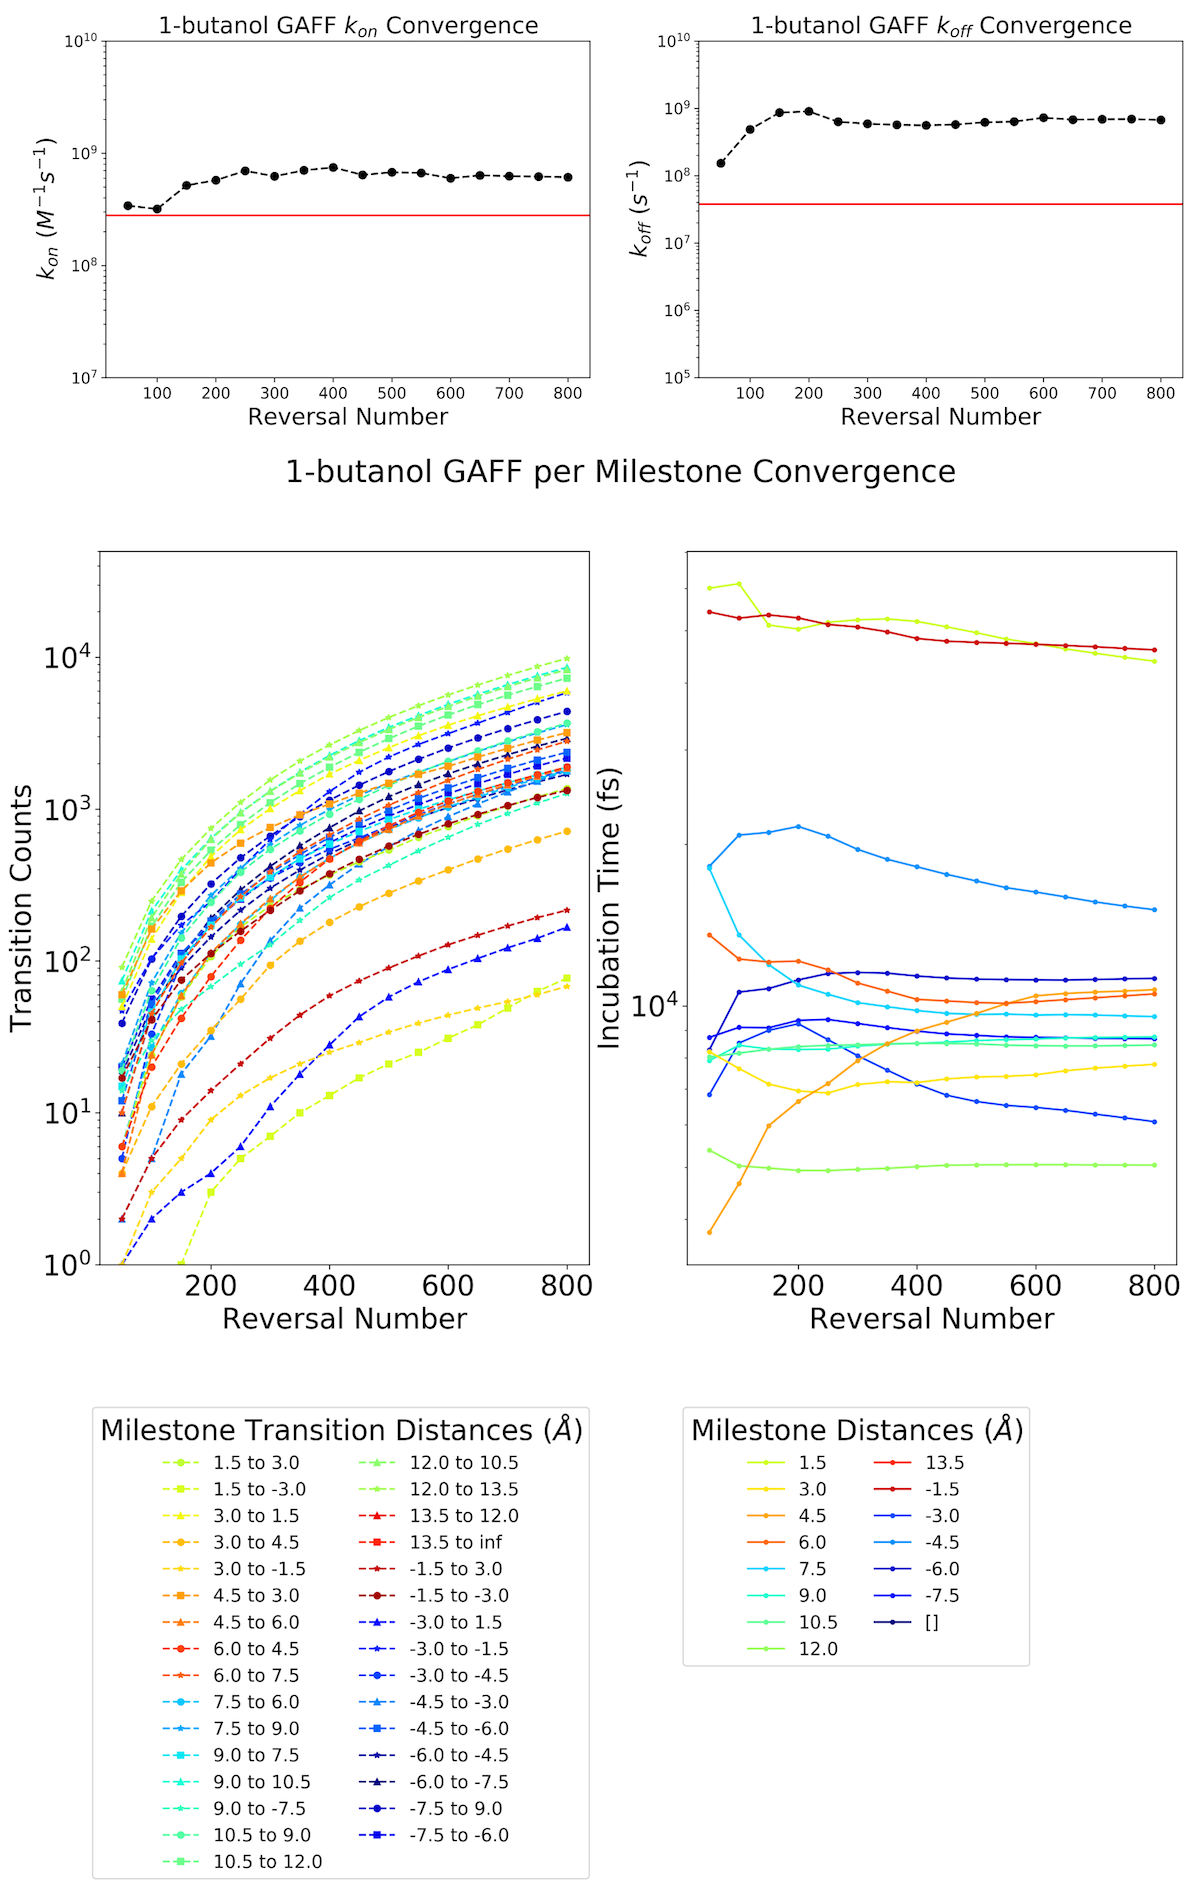
\includegraphics{../images/gaff_convergence_images/1-butanol_gaff_complete.png}
    \caption{1-butanol GAFF per milestone convergence plot}
    \label{fig:1-butanol_gaff_conv}
\end{figure}

\begin{figure}
    %\centering
    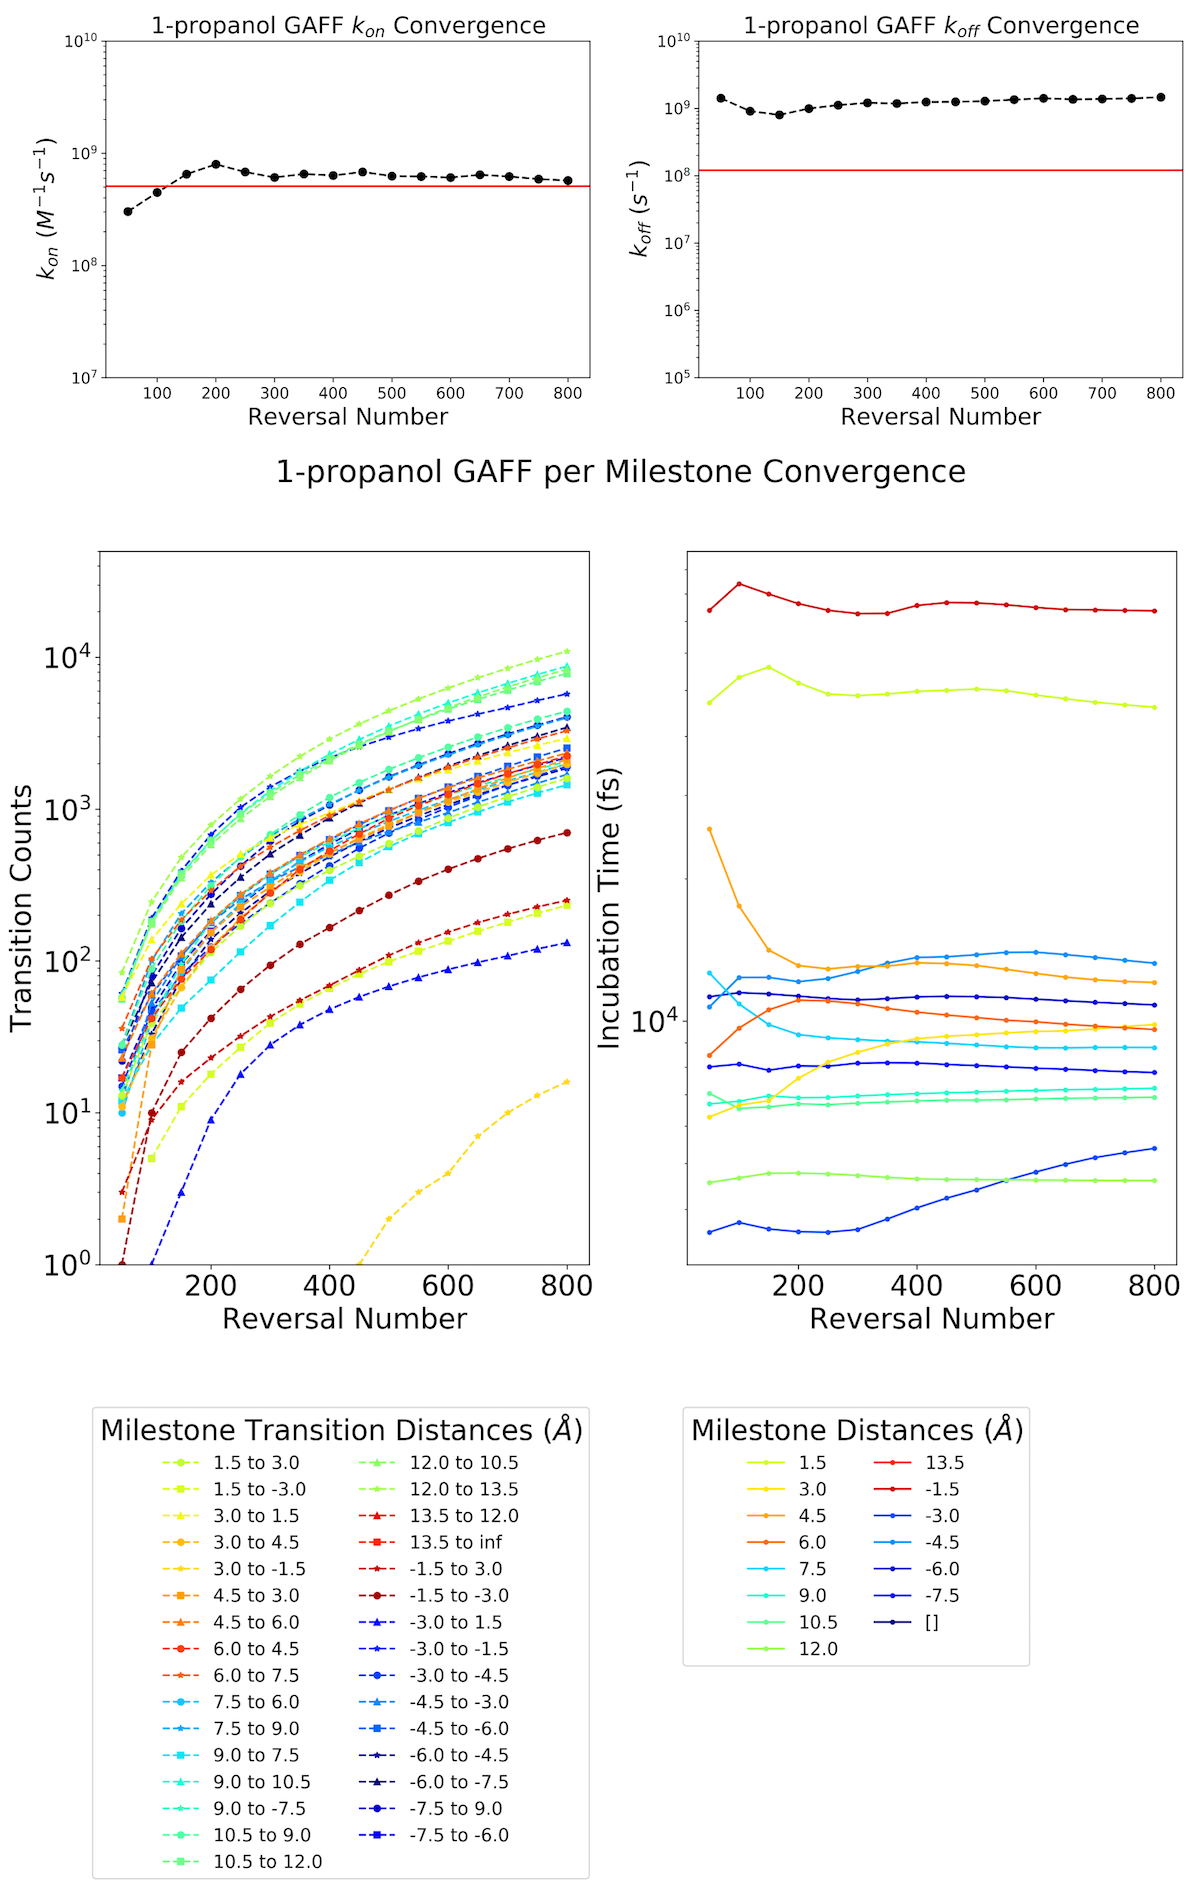
\includegraphics{../images/gaff_convergence_images/1-propanol_gaff_complete.png}
    \caption{1-propanol GAFF per milestone convergence plot}
    \label{fig:1-propanol_gaff_conv}
\end{figure}

\begin{figure}
    %\centering
    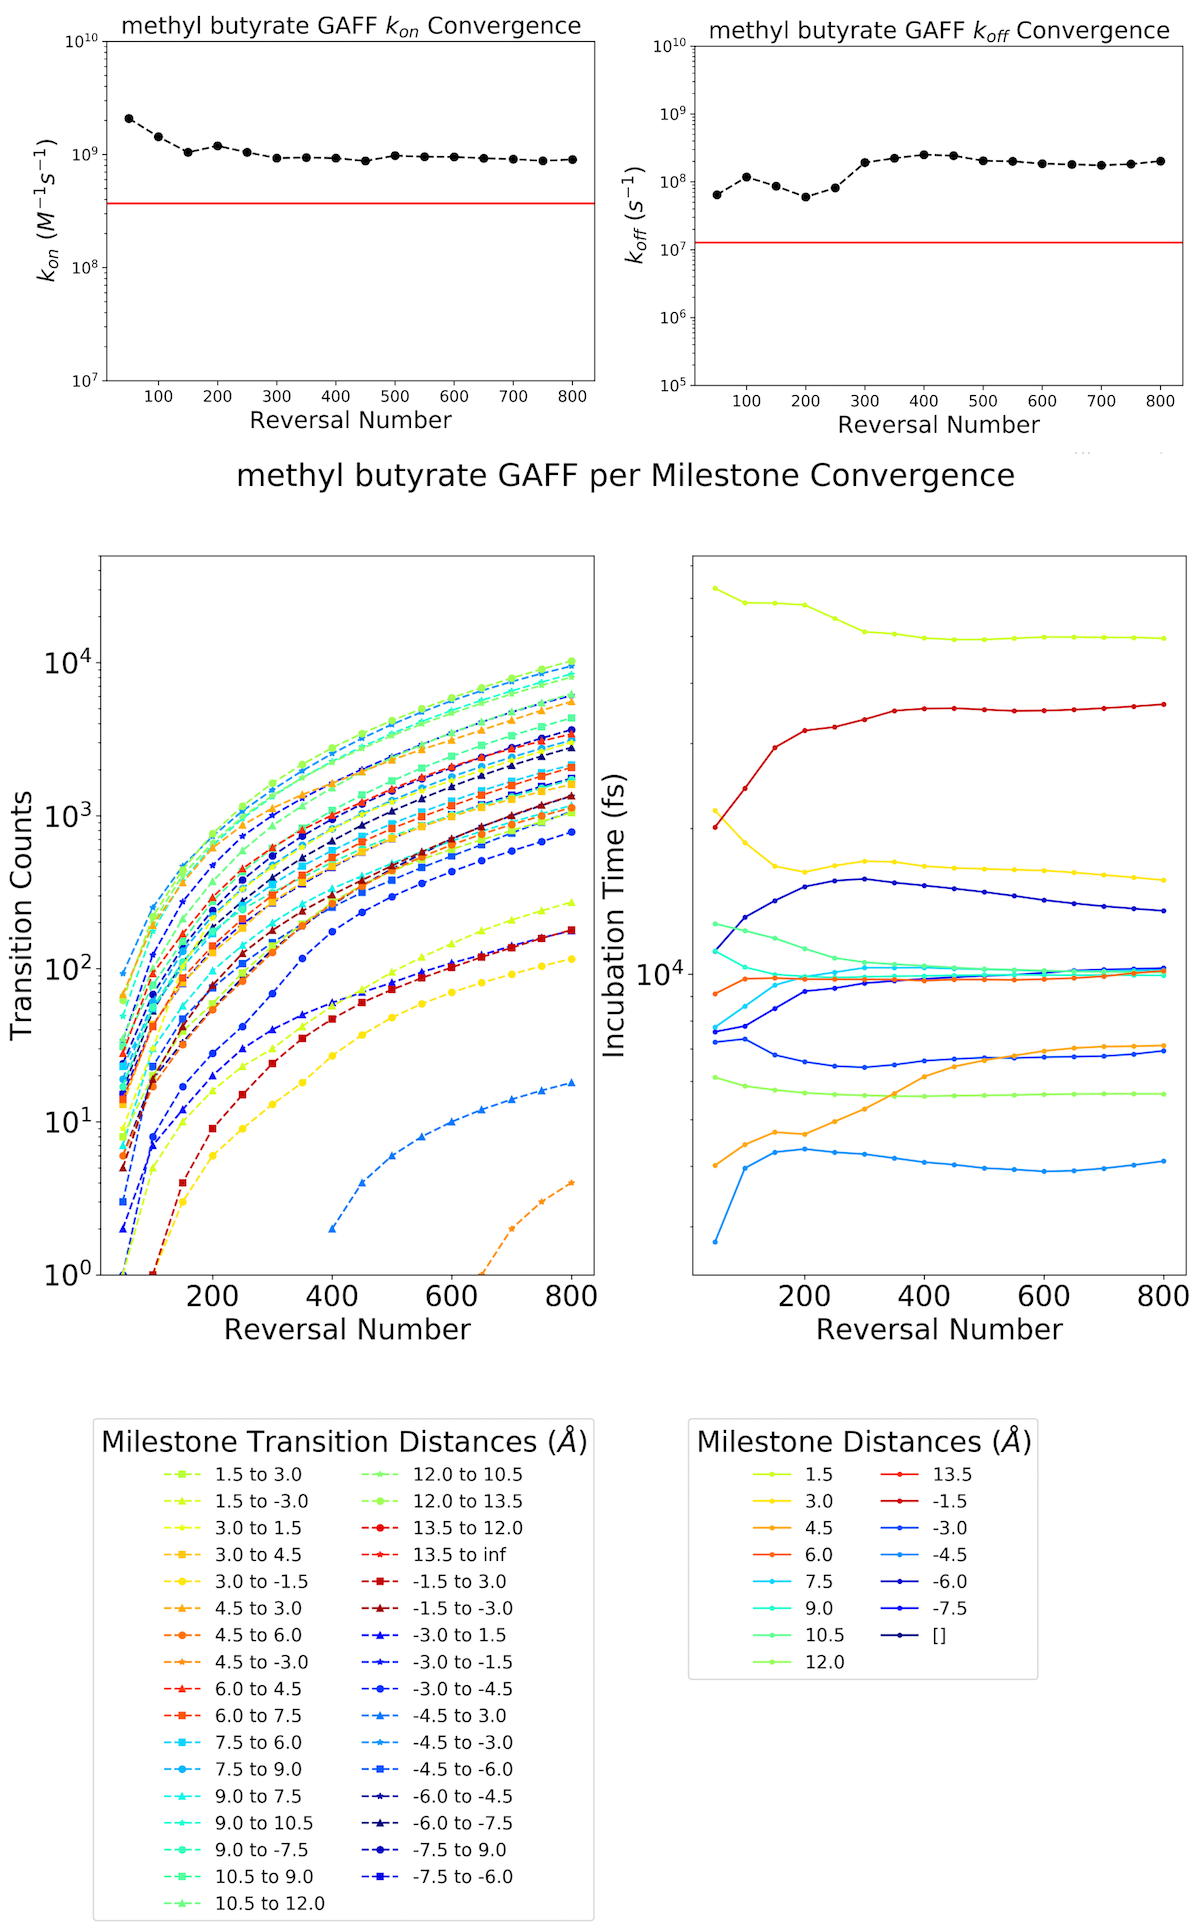
\includegraphics{../images/gaff_convergence_images/methyl_butyrate_gaff_complete.png}
    \caption{methyl butyrate GAFF per milestone convergence plot}
    \label{fig:methyl_butyrate_gaff_conv}
\end{figure}

\begin{figure}
    %\centering
    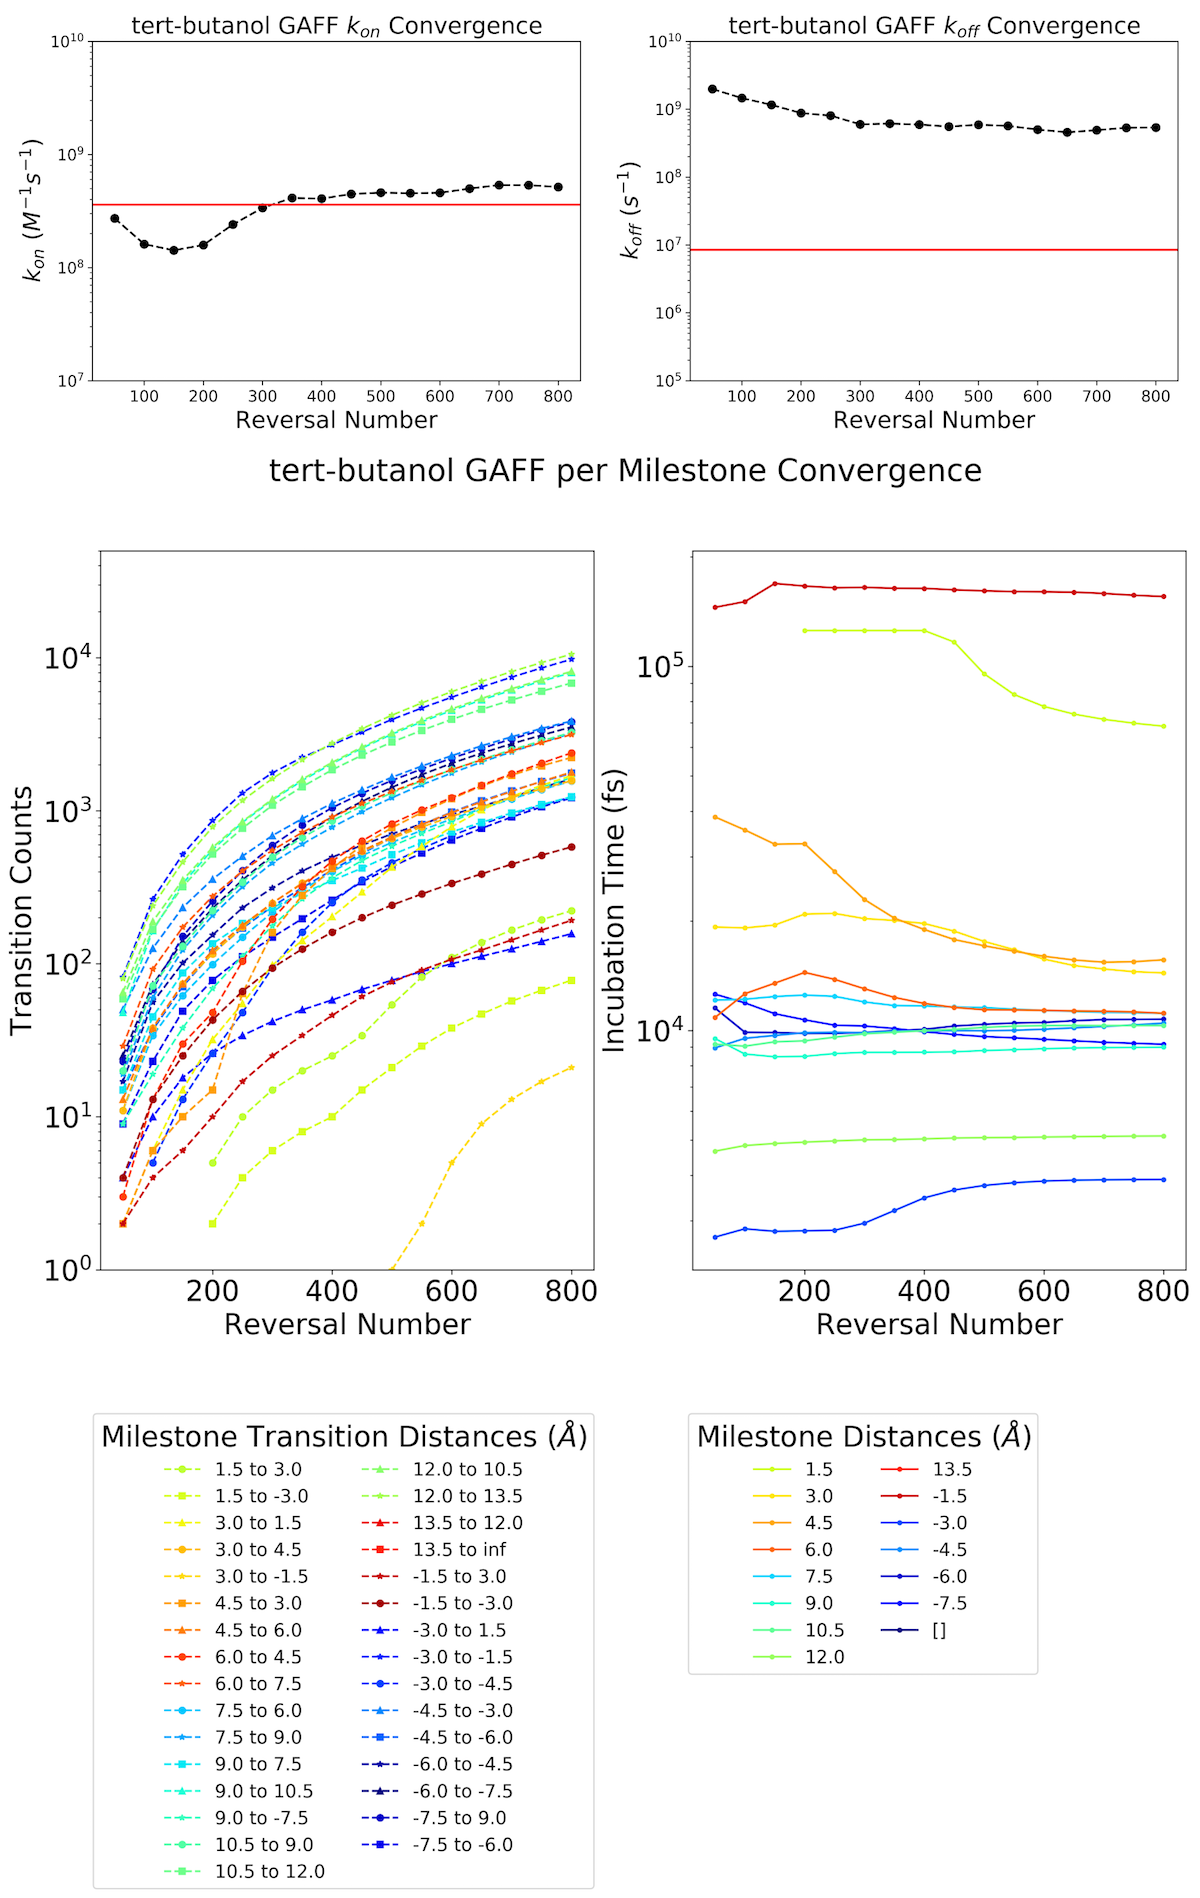
\includegraphics{../images/gaff_convergence_images/tertbutanol_conv_complete.png}
    \caption{tert butanol GAFF per milestone convergence plot}
    \label{fig:tert_butanol_gaff_conv}
\end{figure}

\begin{figure}
    %\centering
    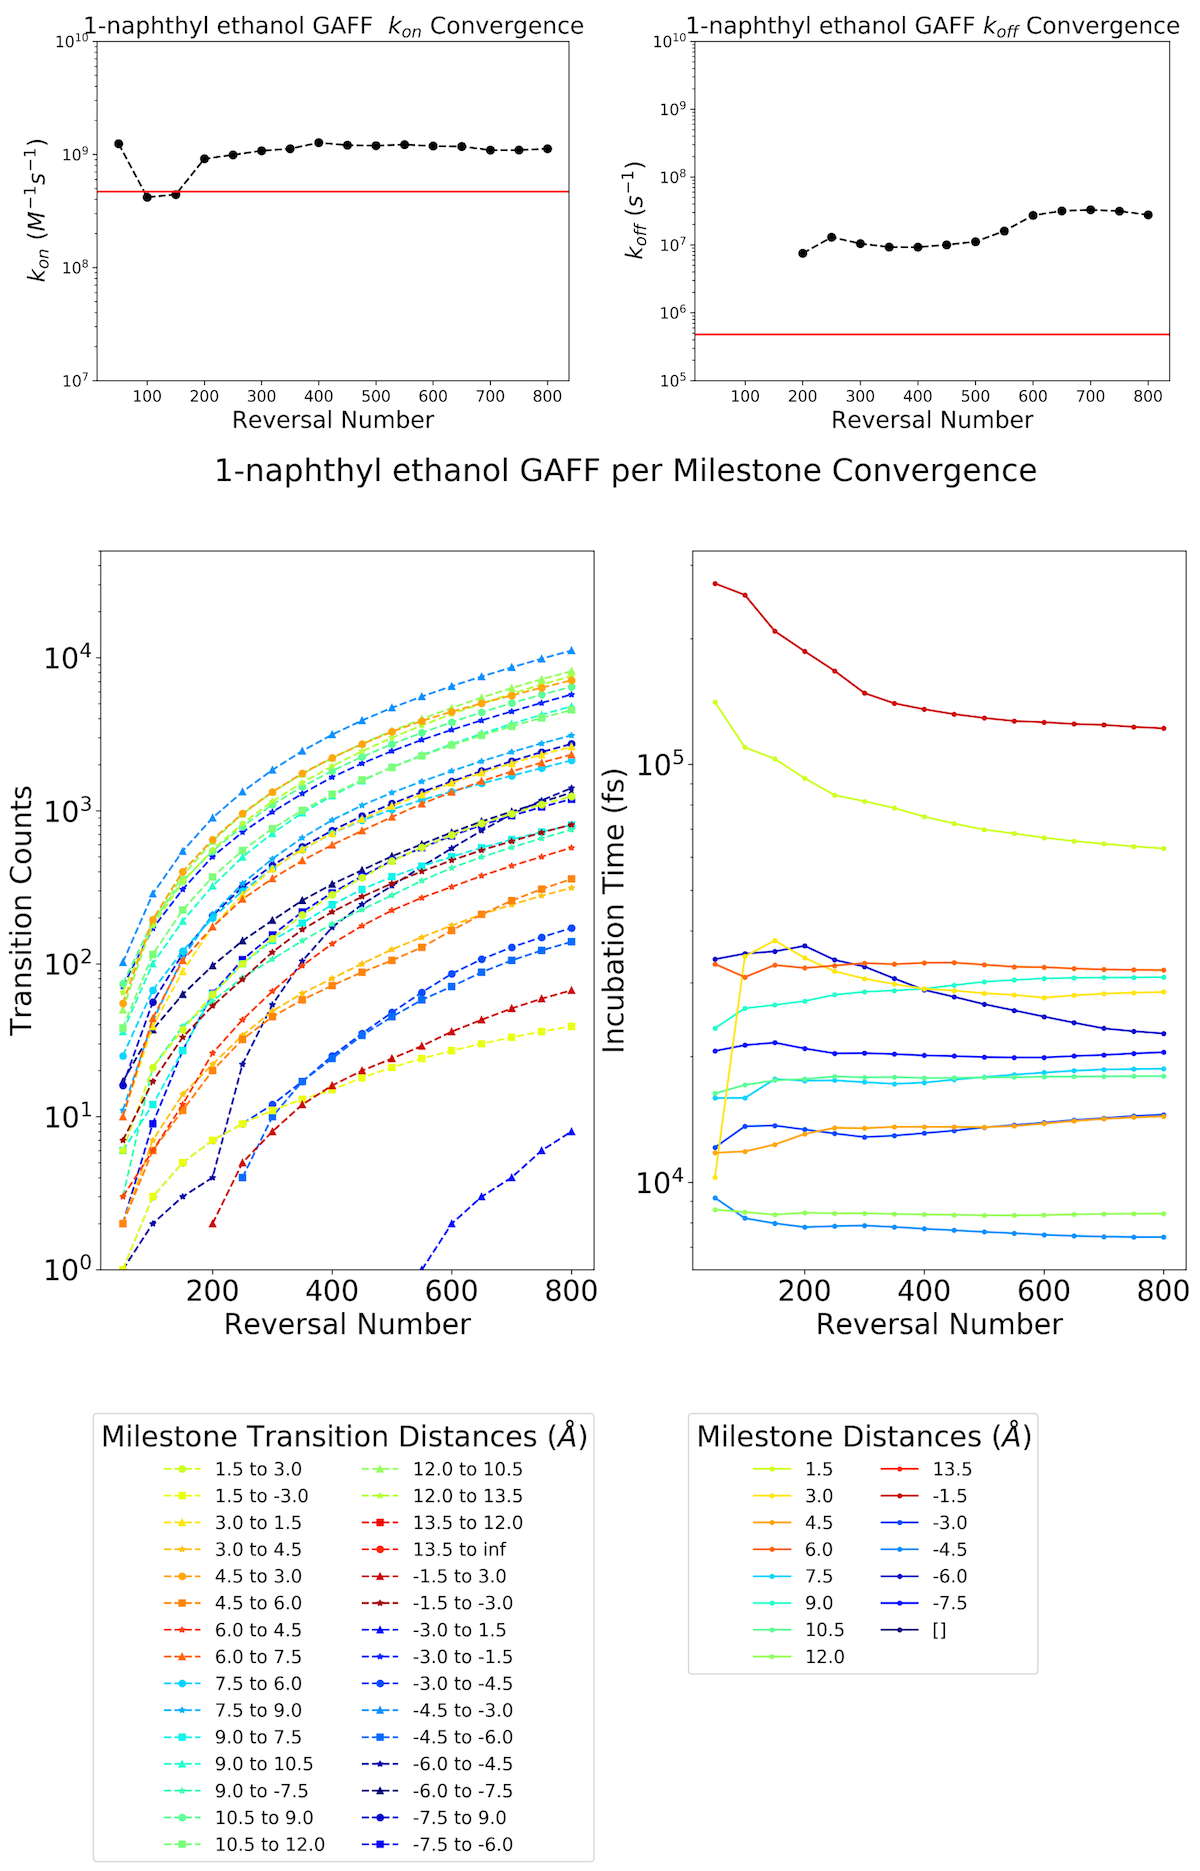
\includegraphics{../images/gaff_convergence_images/1-naphthylethanol_gaff_complete.png}
    \caption{1-naphthyl ethanol GAFF per milestone convergence plot}
    \label{fig:1-naphthylethanol_gaff_conv}
\end{figure}

\begin{figure}
    %\centering
    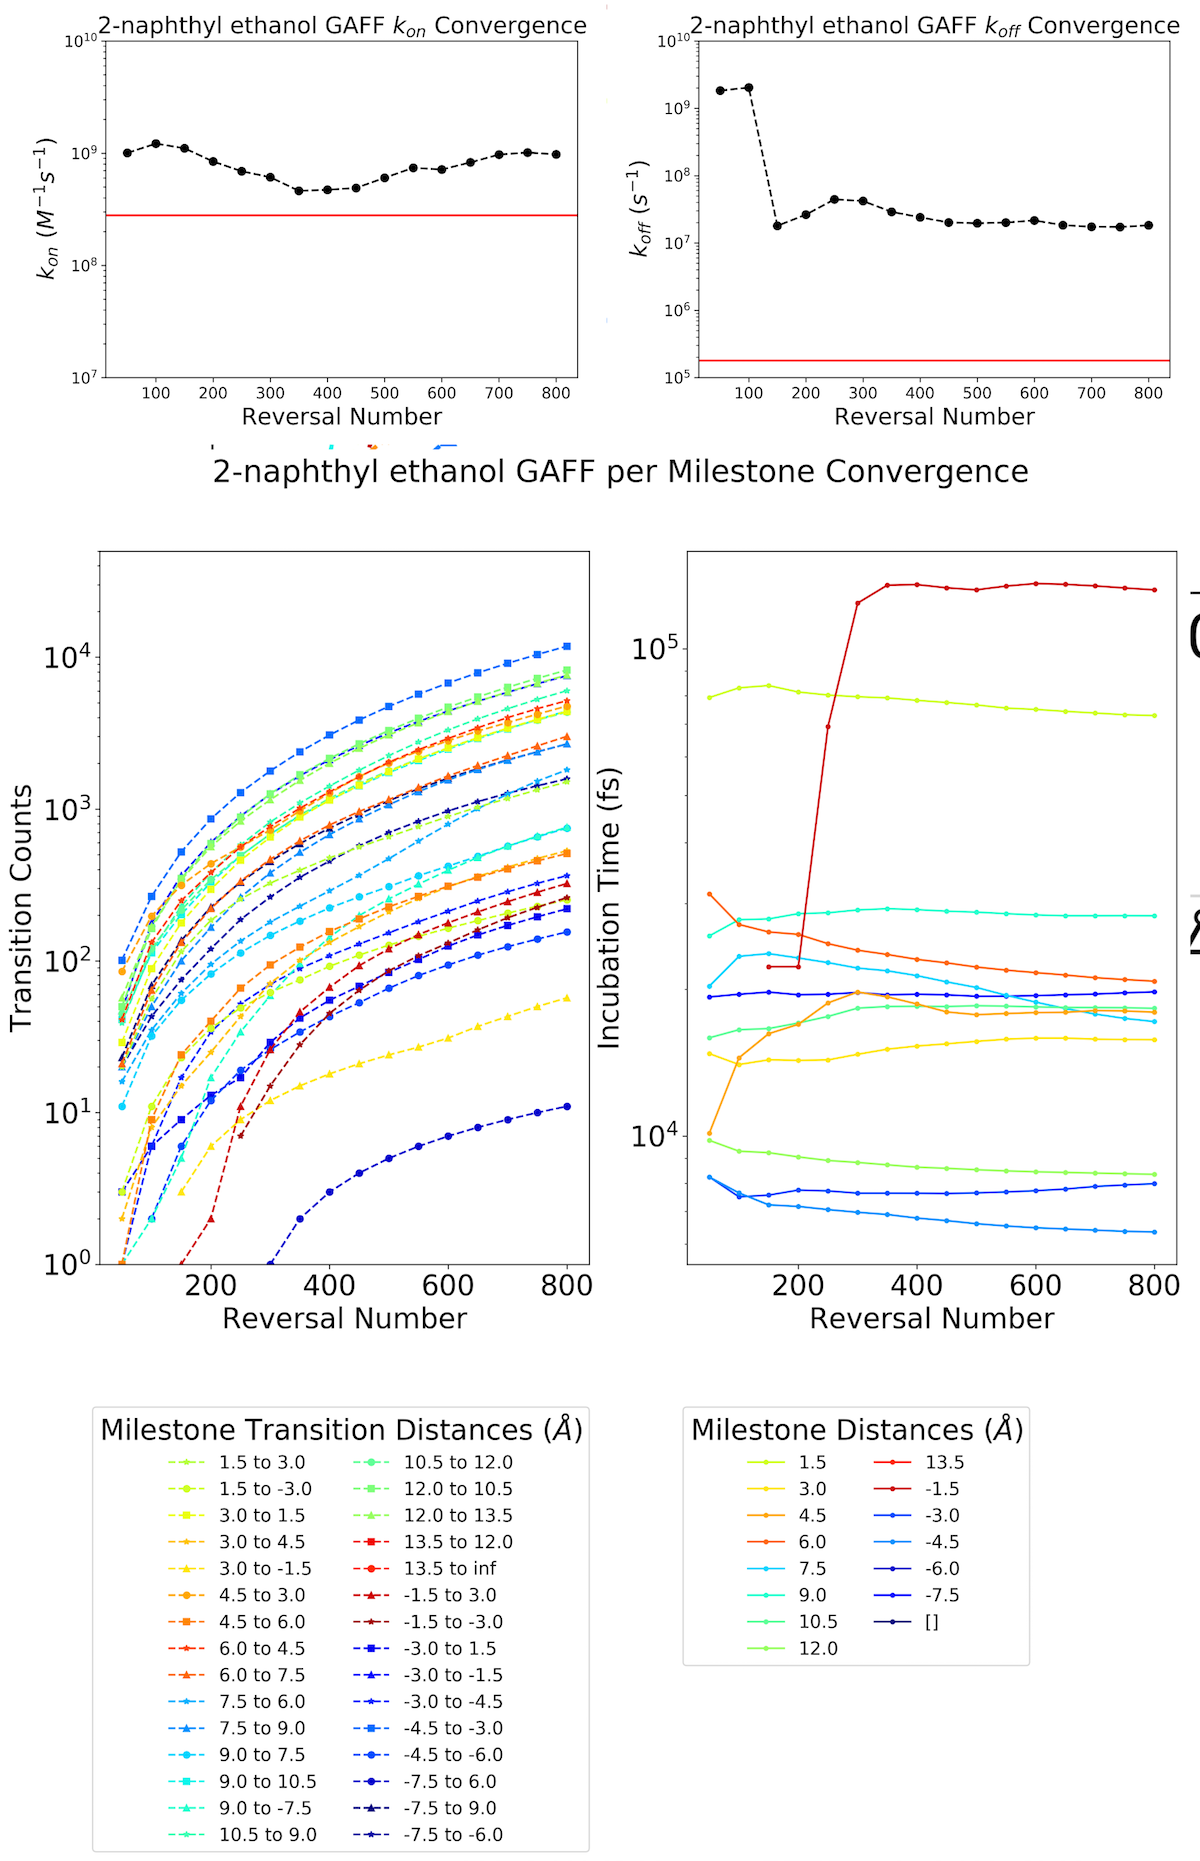
\includegraphics{../images/gaff_convergence_images/2-naphthylethanol_gaff_complete.png}
    \caption{2-naphthyl ethanol GAFF per milestone convergence plot}
    \label{fig:2-naphthylethanol_gaff_conv}
\end{figure}

\begin{figure}
    %\centering
    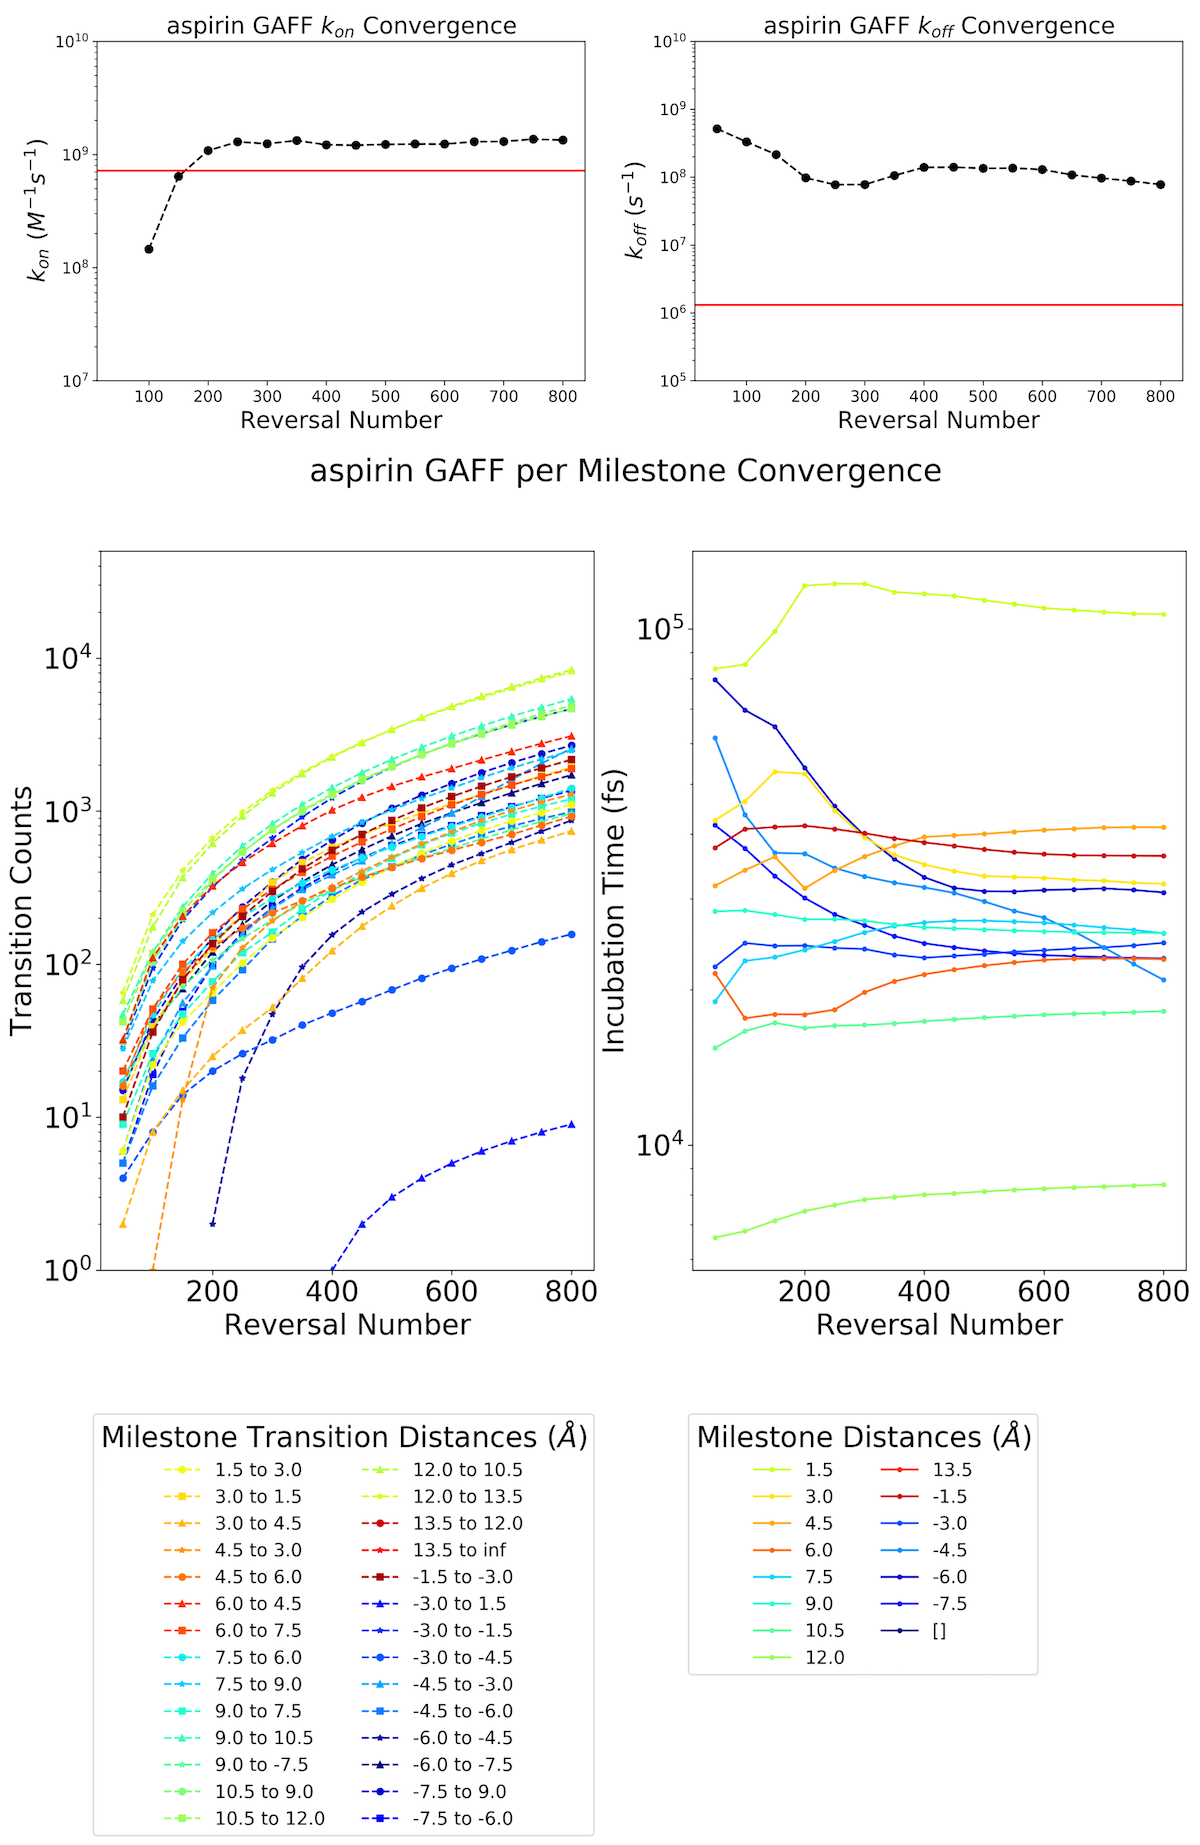
\includegraphics{../images/gaff_convergence_images/aspirin_gaff_complete.png}
    \caption{aspirin GAFF per milestone convergence plot}
    \label{fig:aspirin_conv}
\end{figure}






\begin{figure}
    %\centering
    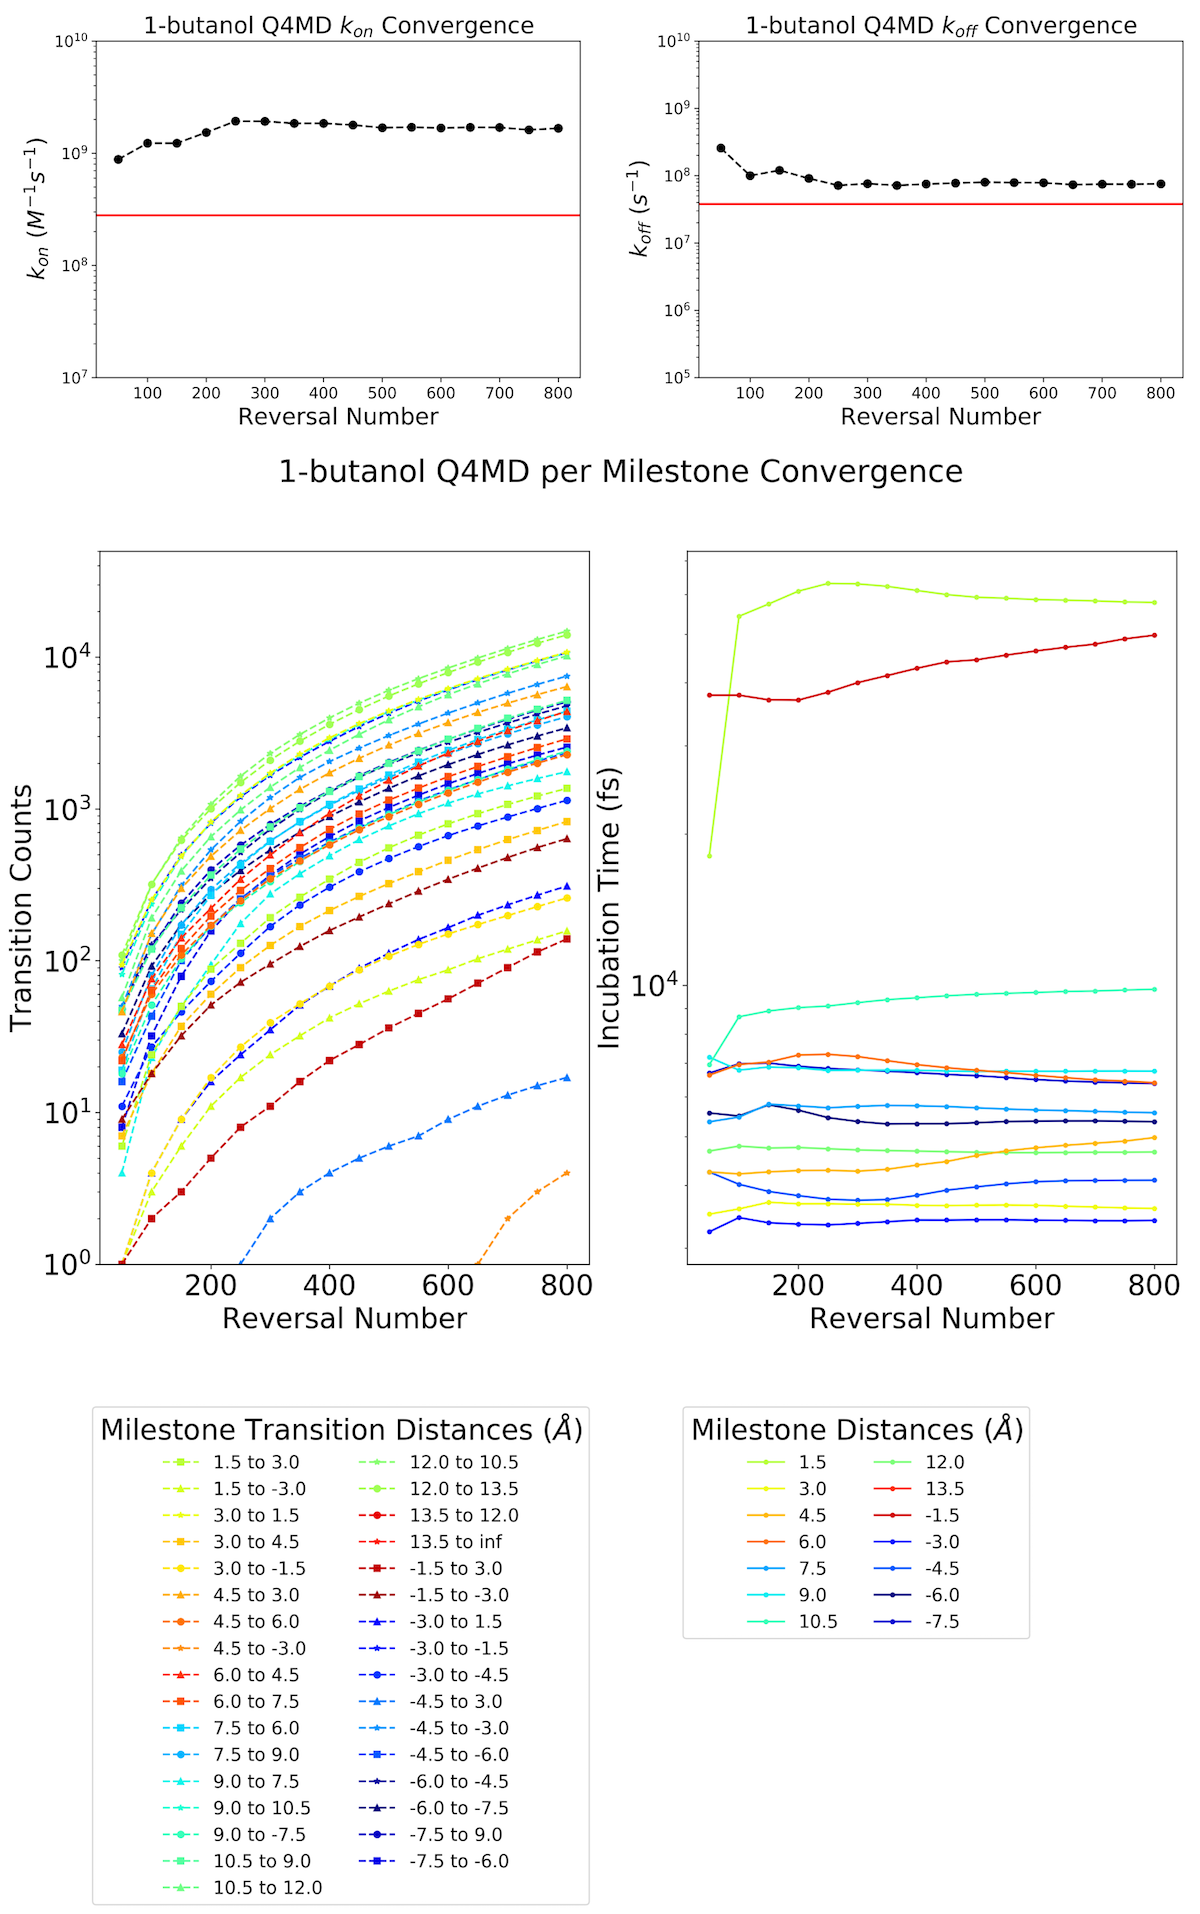
\includegraphics{../images/q4md_convergence_images/1-butanol_q4md_complete.png}
    \caption{1-butanol Q4MD per milestone convergence plot}
    \label{fig:1-butanol_q4md_conv}
\end{figure}

\begin{figure}
    %\centering
    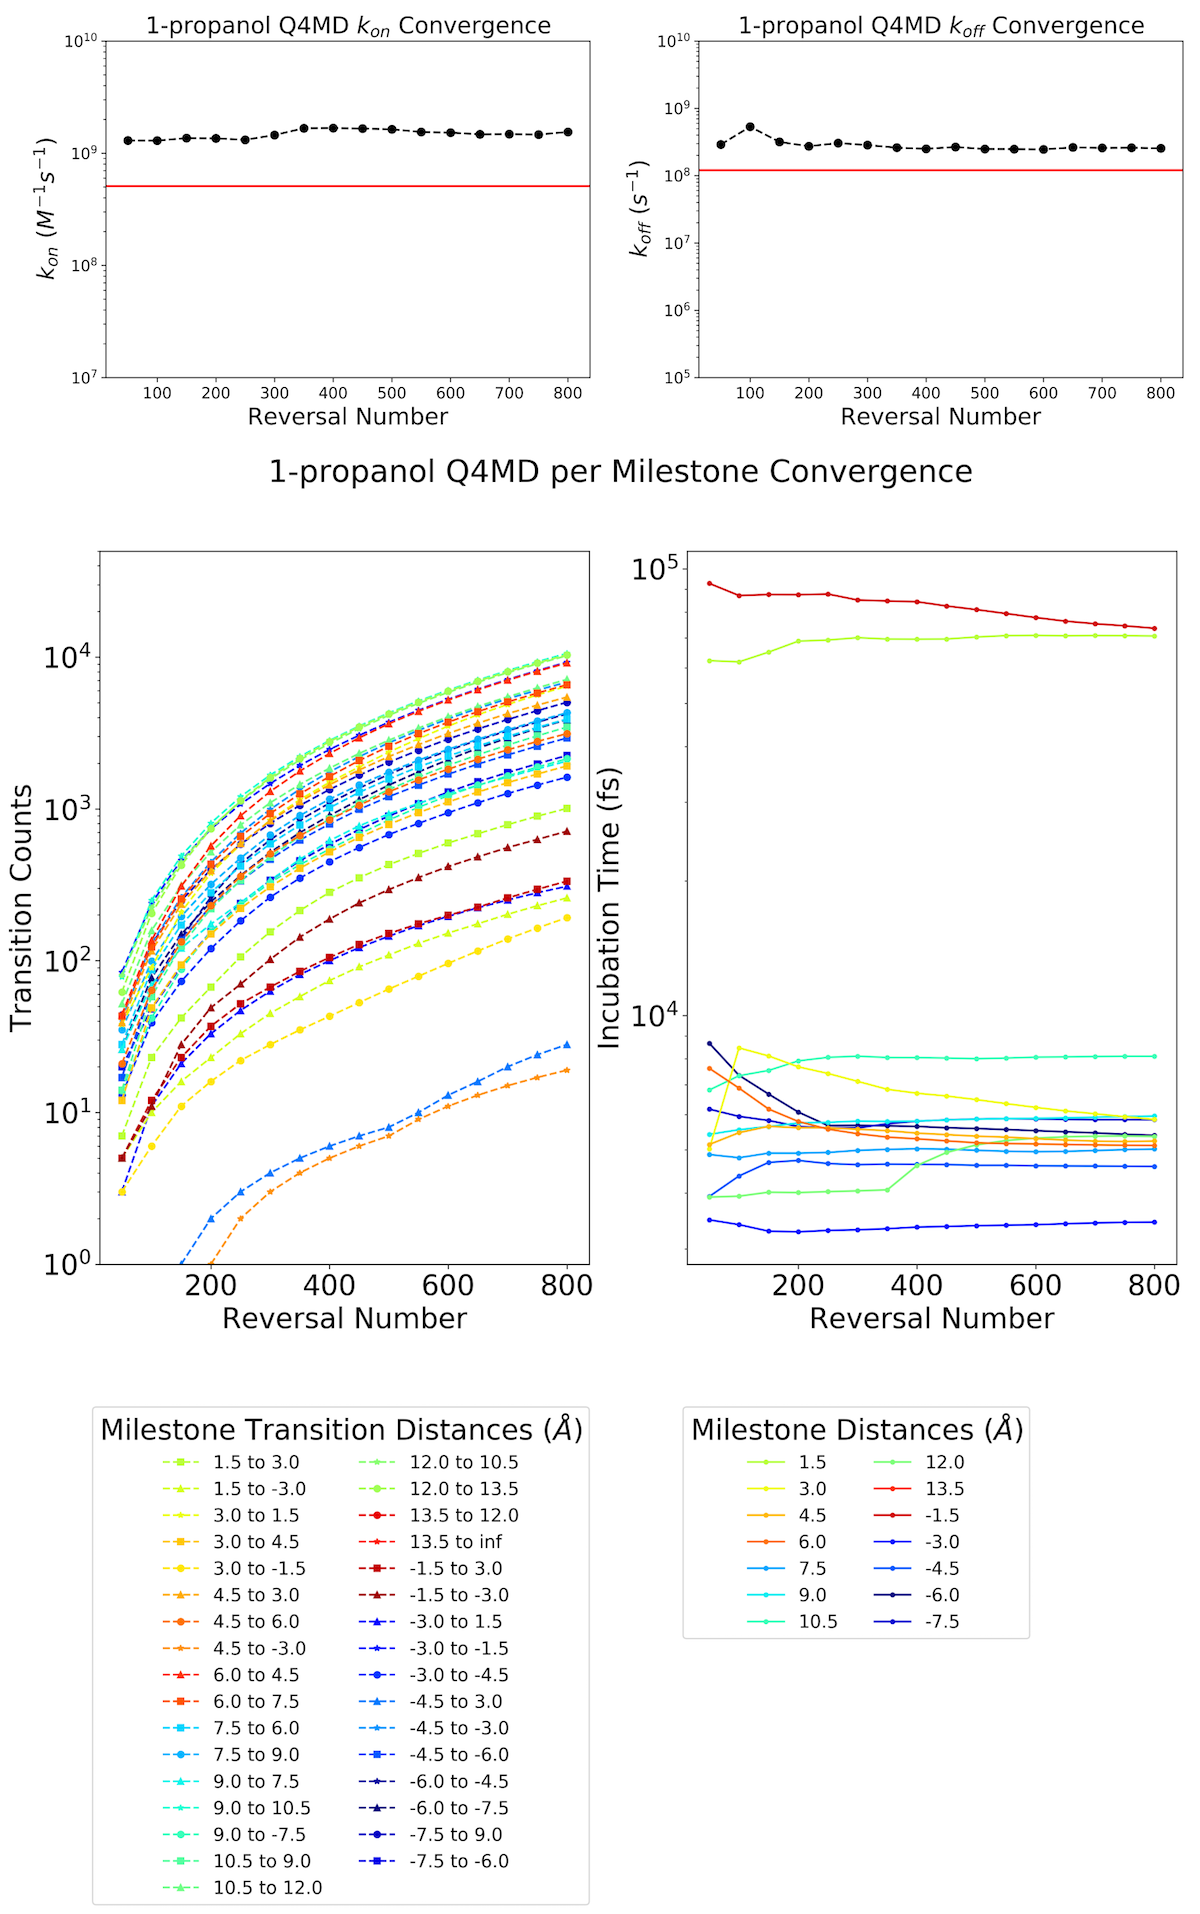
\includegraphics{../images/q4md_convergence_images/1-propanol_q4md_complete.png}
    \caption{1-propanol Q4MD per milestone convergence plot}
    \label{fig:1-propanol_q4md_conv}
\end{figure}

\begin{figure}
    %\centering
    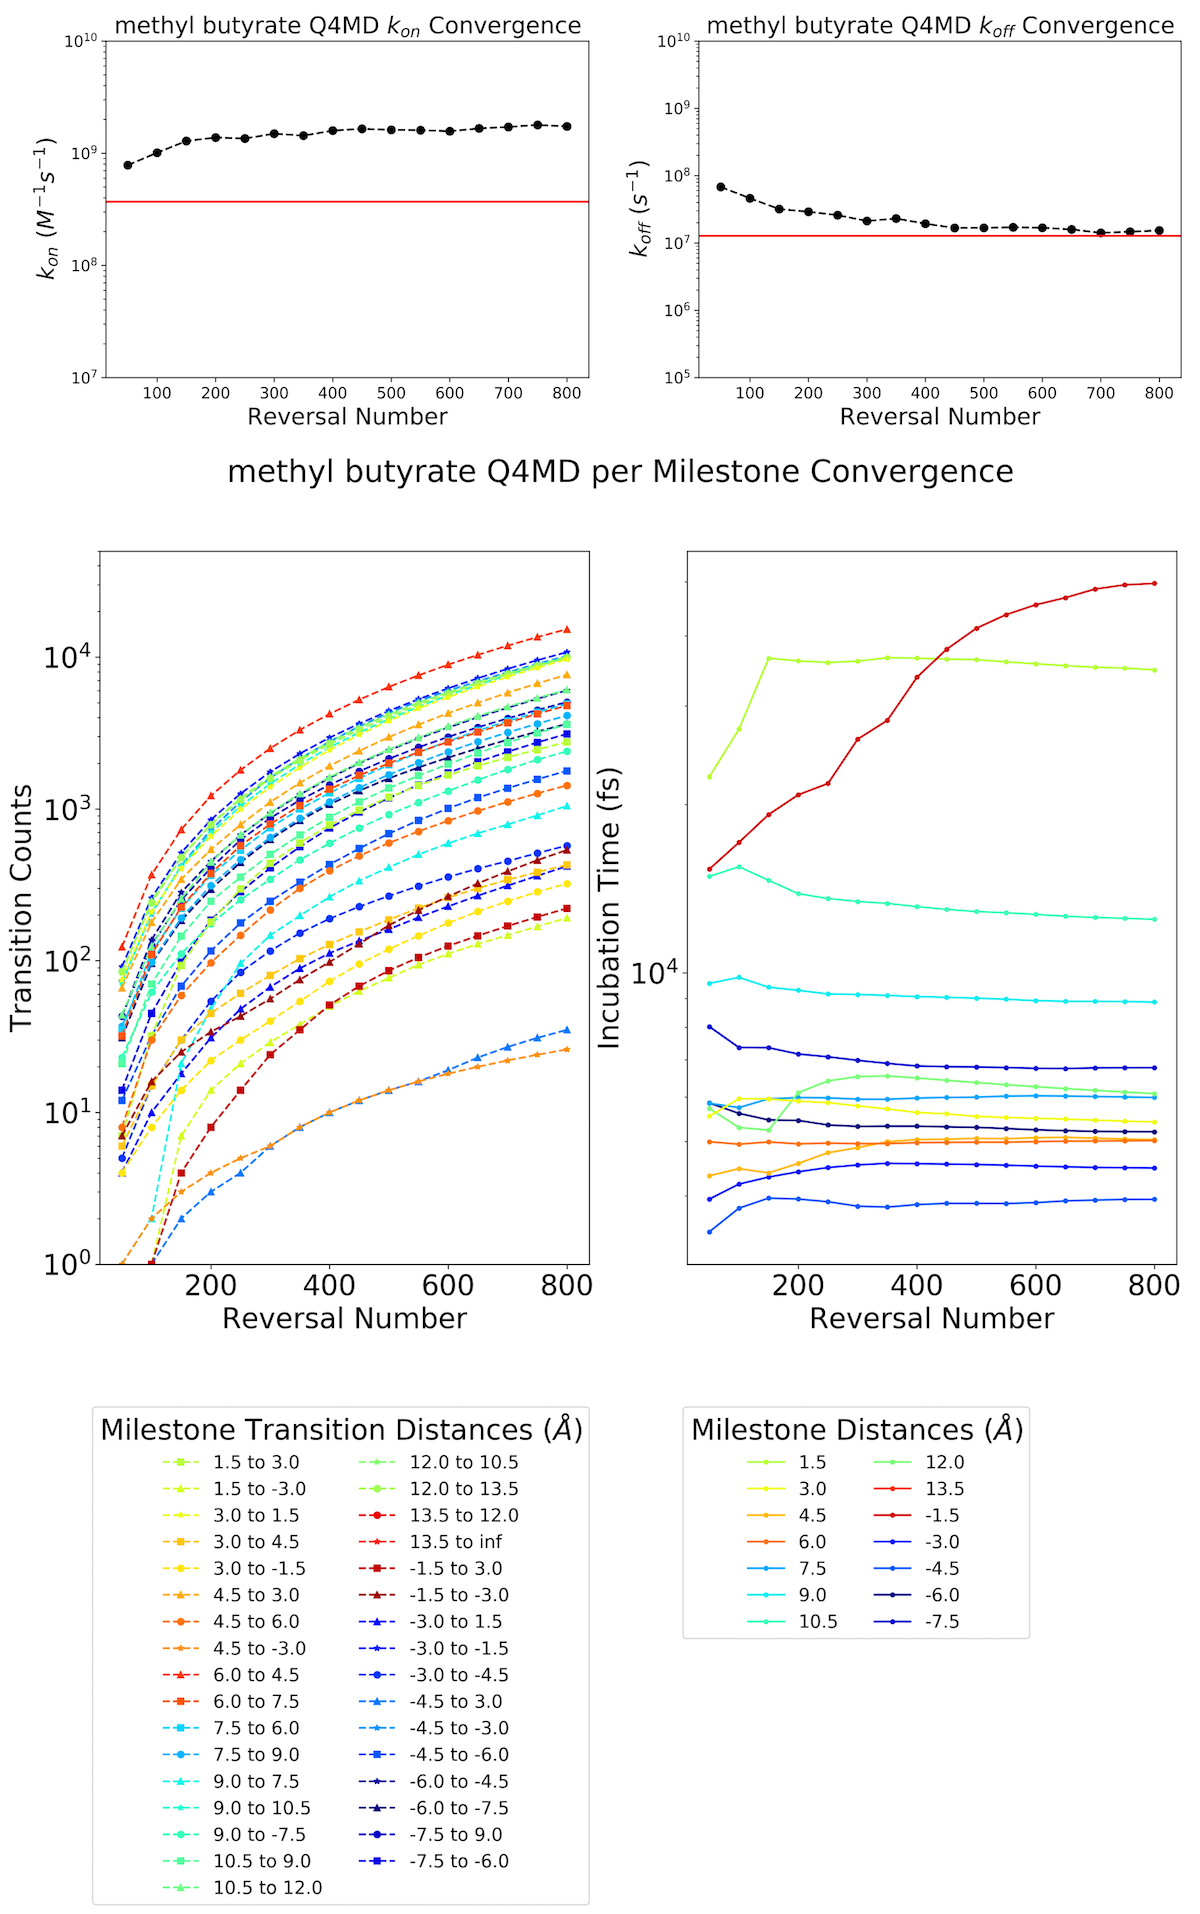
\includegraphics{../images/q4md_convergence_images/methyl_butyrate_q4md_complete.png}
    \caption{methyl butyrate Q4MD per milestone convergence plot}
    \label{fig:methyl_butyrate_q4md_conv}
\end{figure}

\begin{figure}
    %\centering
    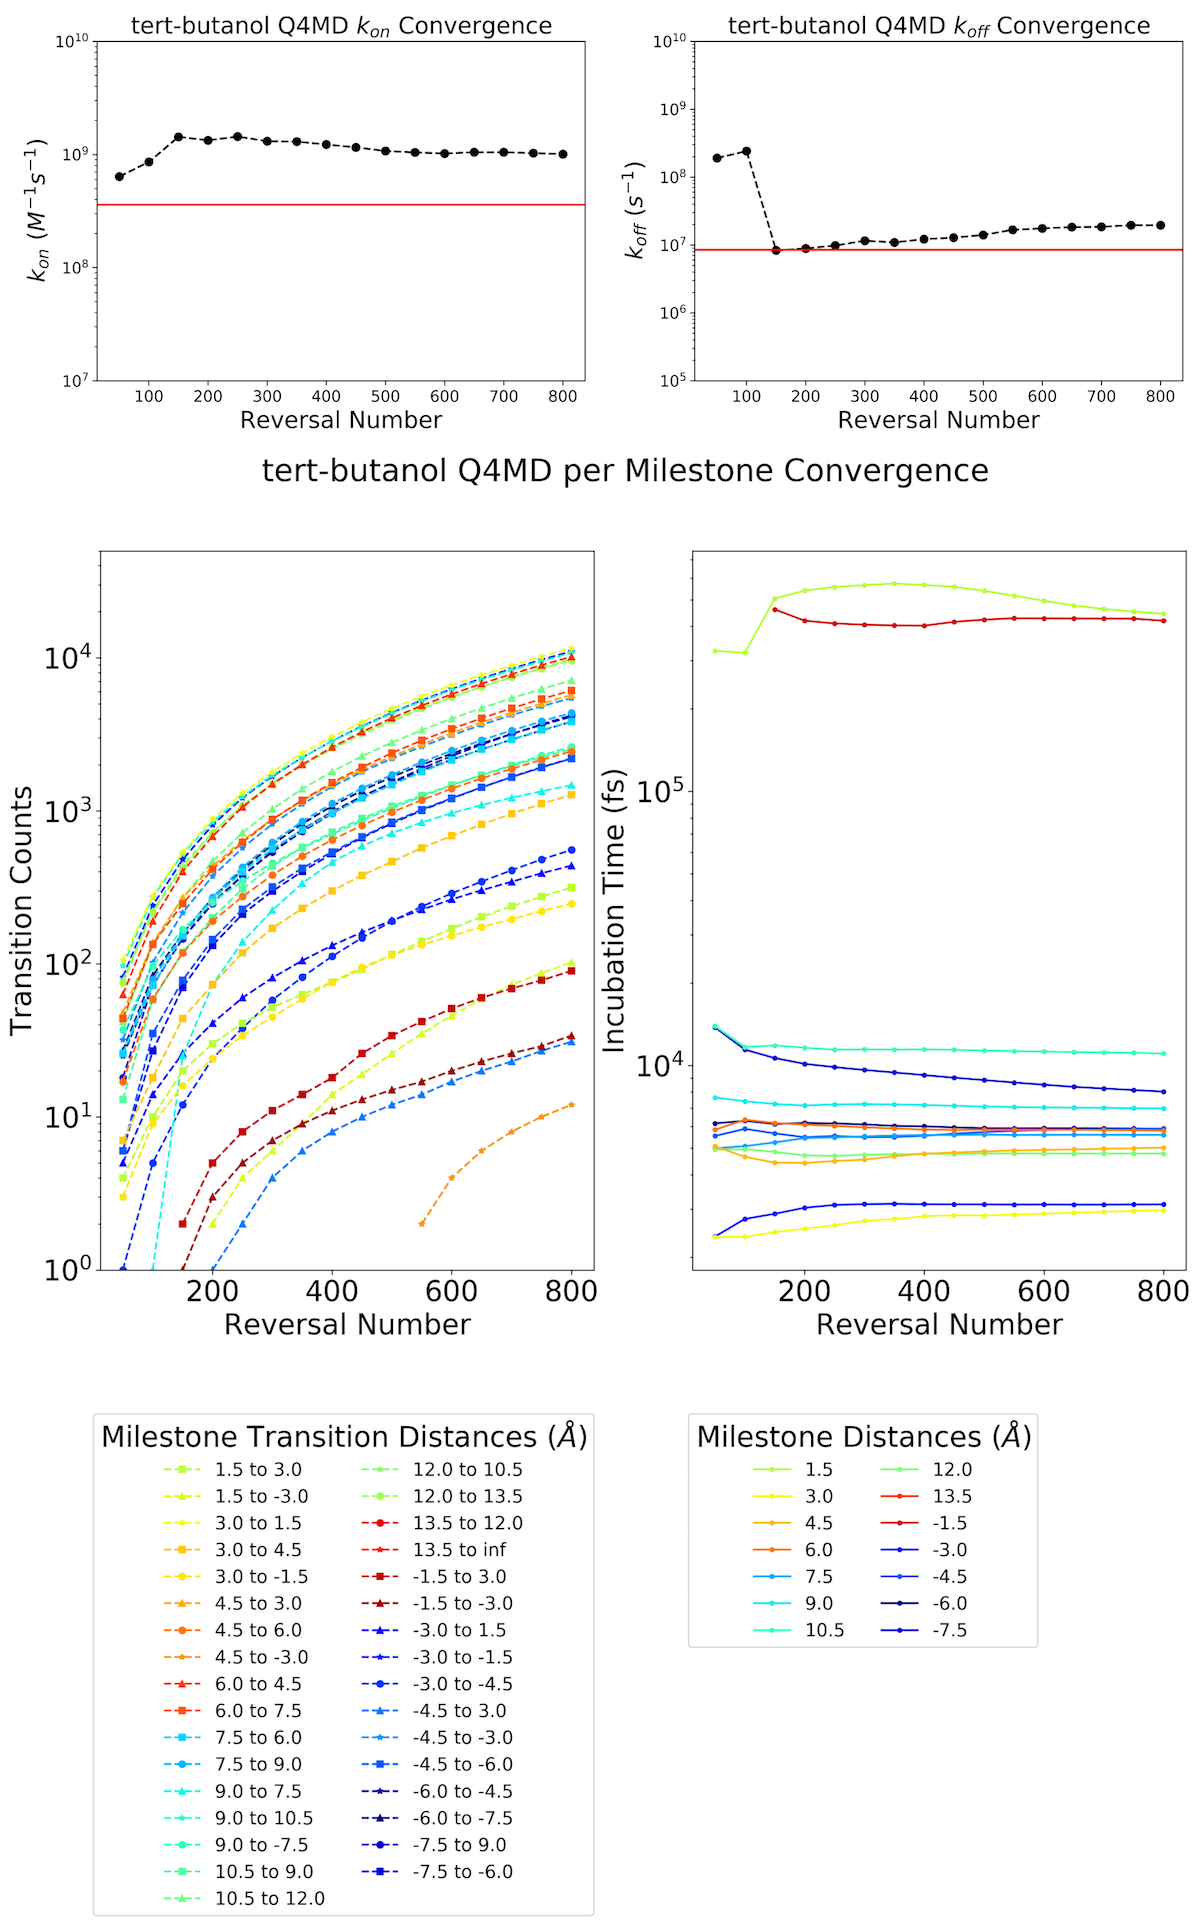
\includegraphics{../images/q4md_convergence_images/tertbutanol_q4md_complete.png}
    \caption{tert butanol Q4MD per milestone convergence plot}
    \label{fig:tert_butanol_q4md_conv}
\end{figure}

\begin{figure}
    %\centering
    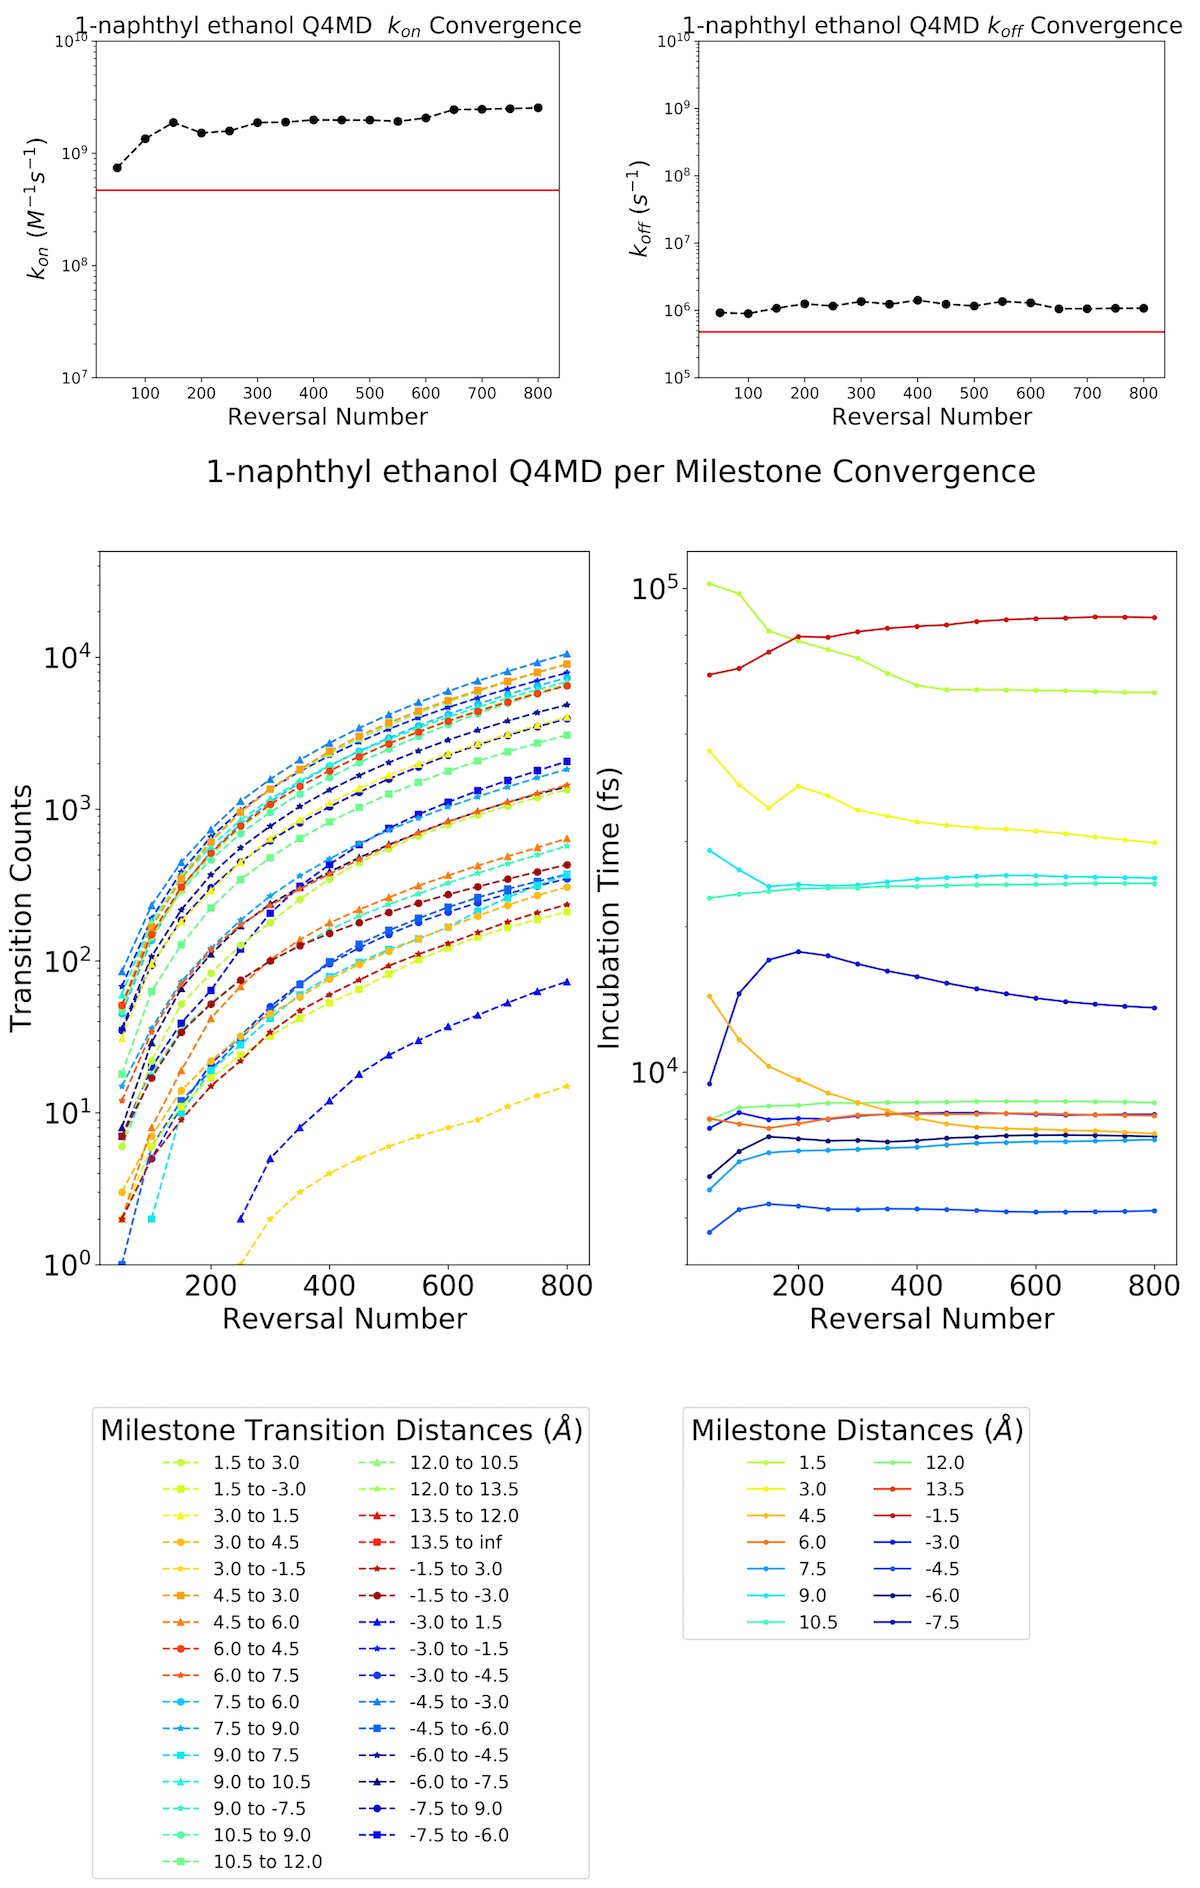
\includegraphics{../images/q4md_convergence_images/1-naphthylethanol_q4md_complete.png}
    \caption{1-naphthyl ethanol Q4MD per milestone convergence plot}
    \label{fig:1-naphthylethanol_q4md_conv}
\end{figure}

\begin{figure}
    %\centering
    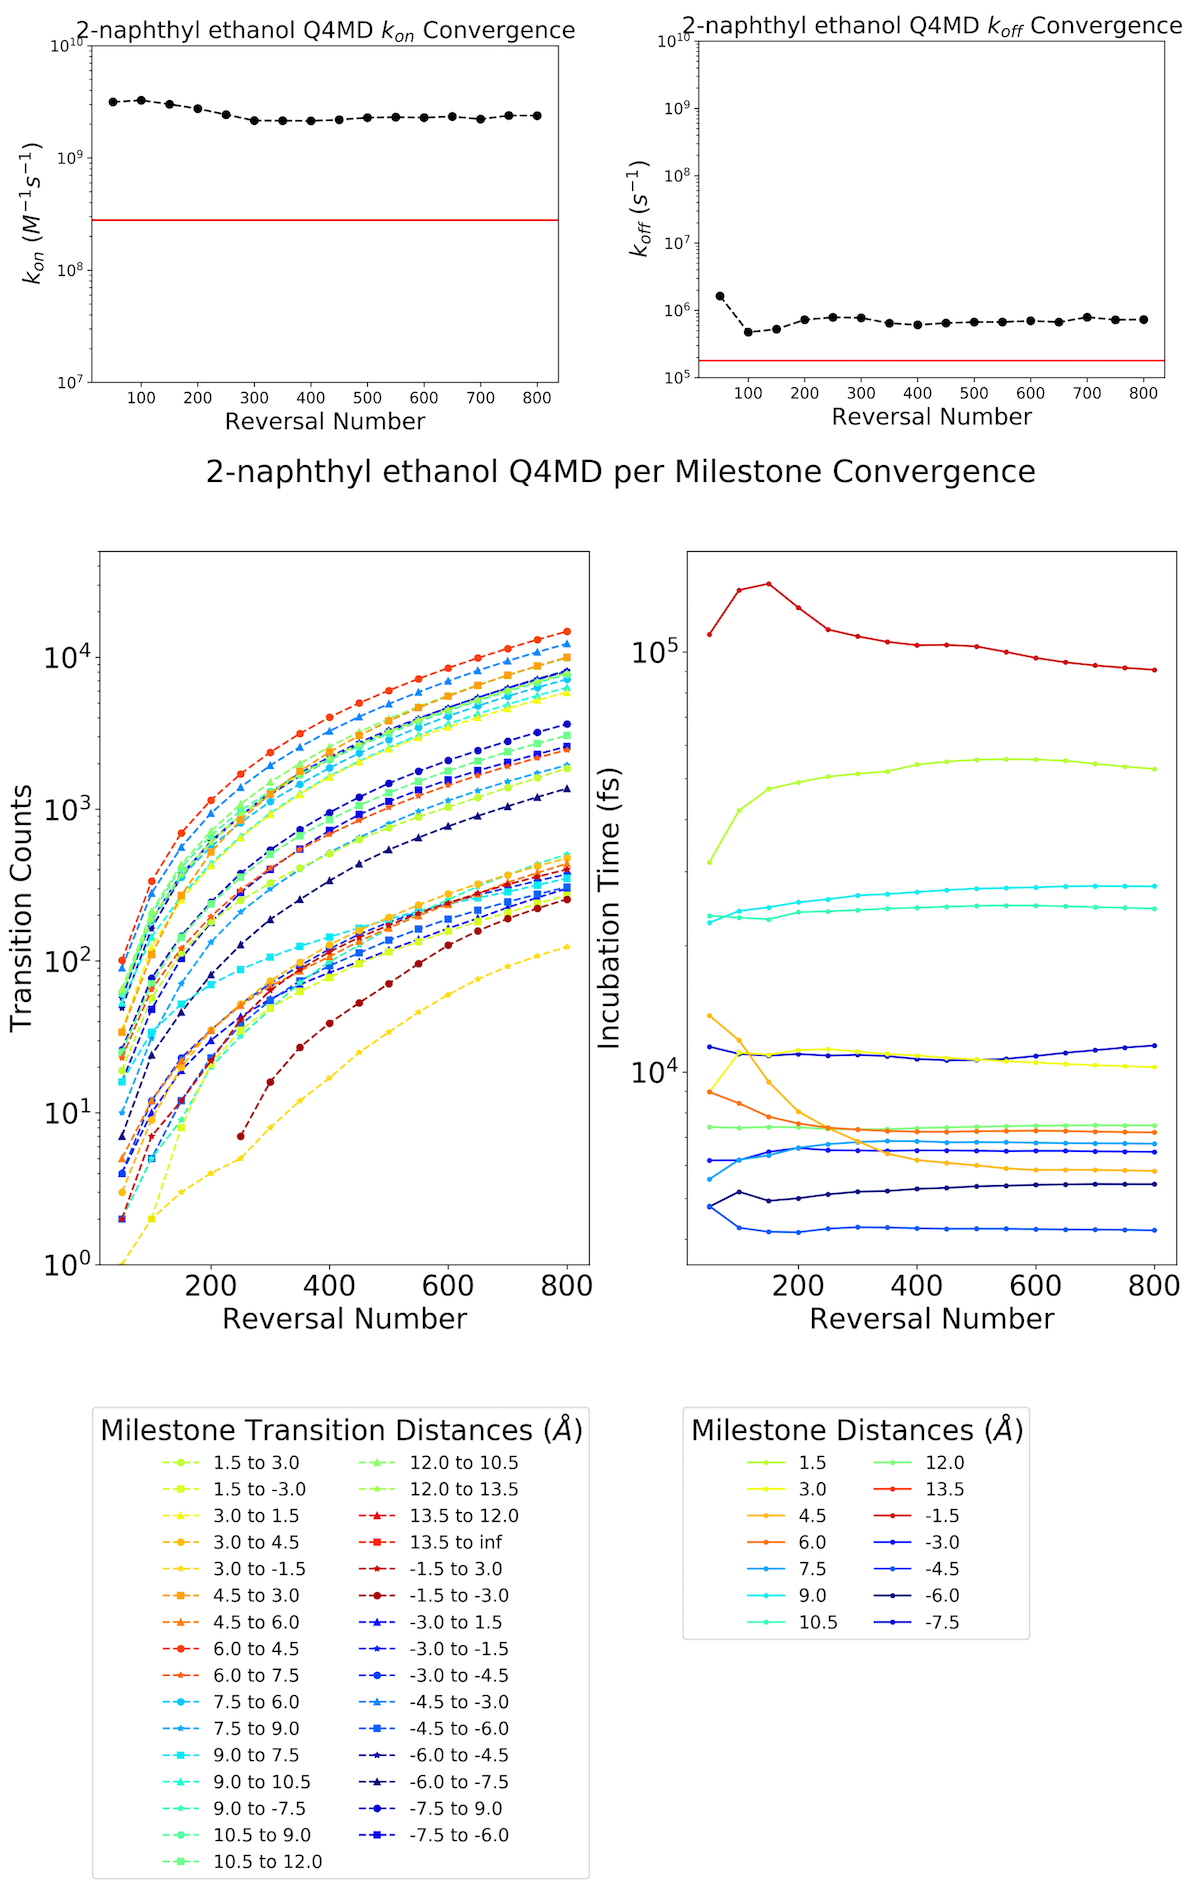
\includegraphics{../images/q4md_convergence_images/2-naphthylethanol_q4md_complete.png}
    \caption{2-naphthyl ethanol Q4MD per milestone convergence plot}
    \label{fig:2-naphthylethanol_q4md_conv}
\end{figure}

\begin{figure}
    %\centering
    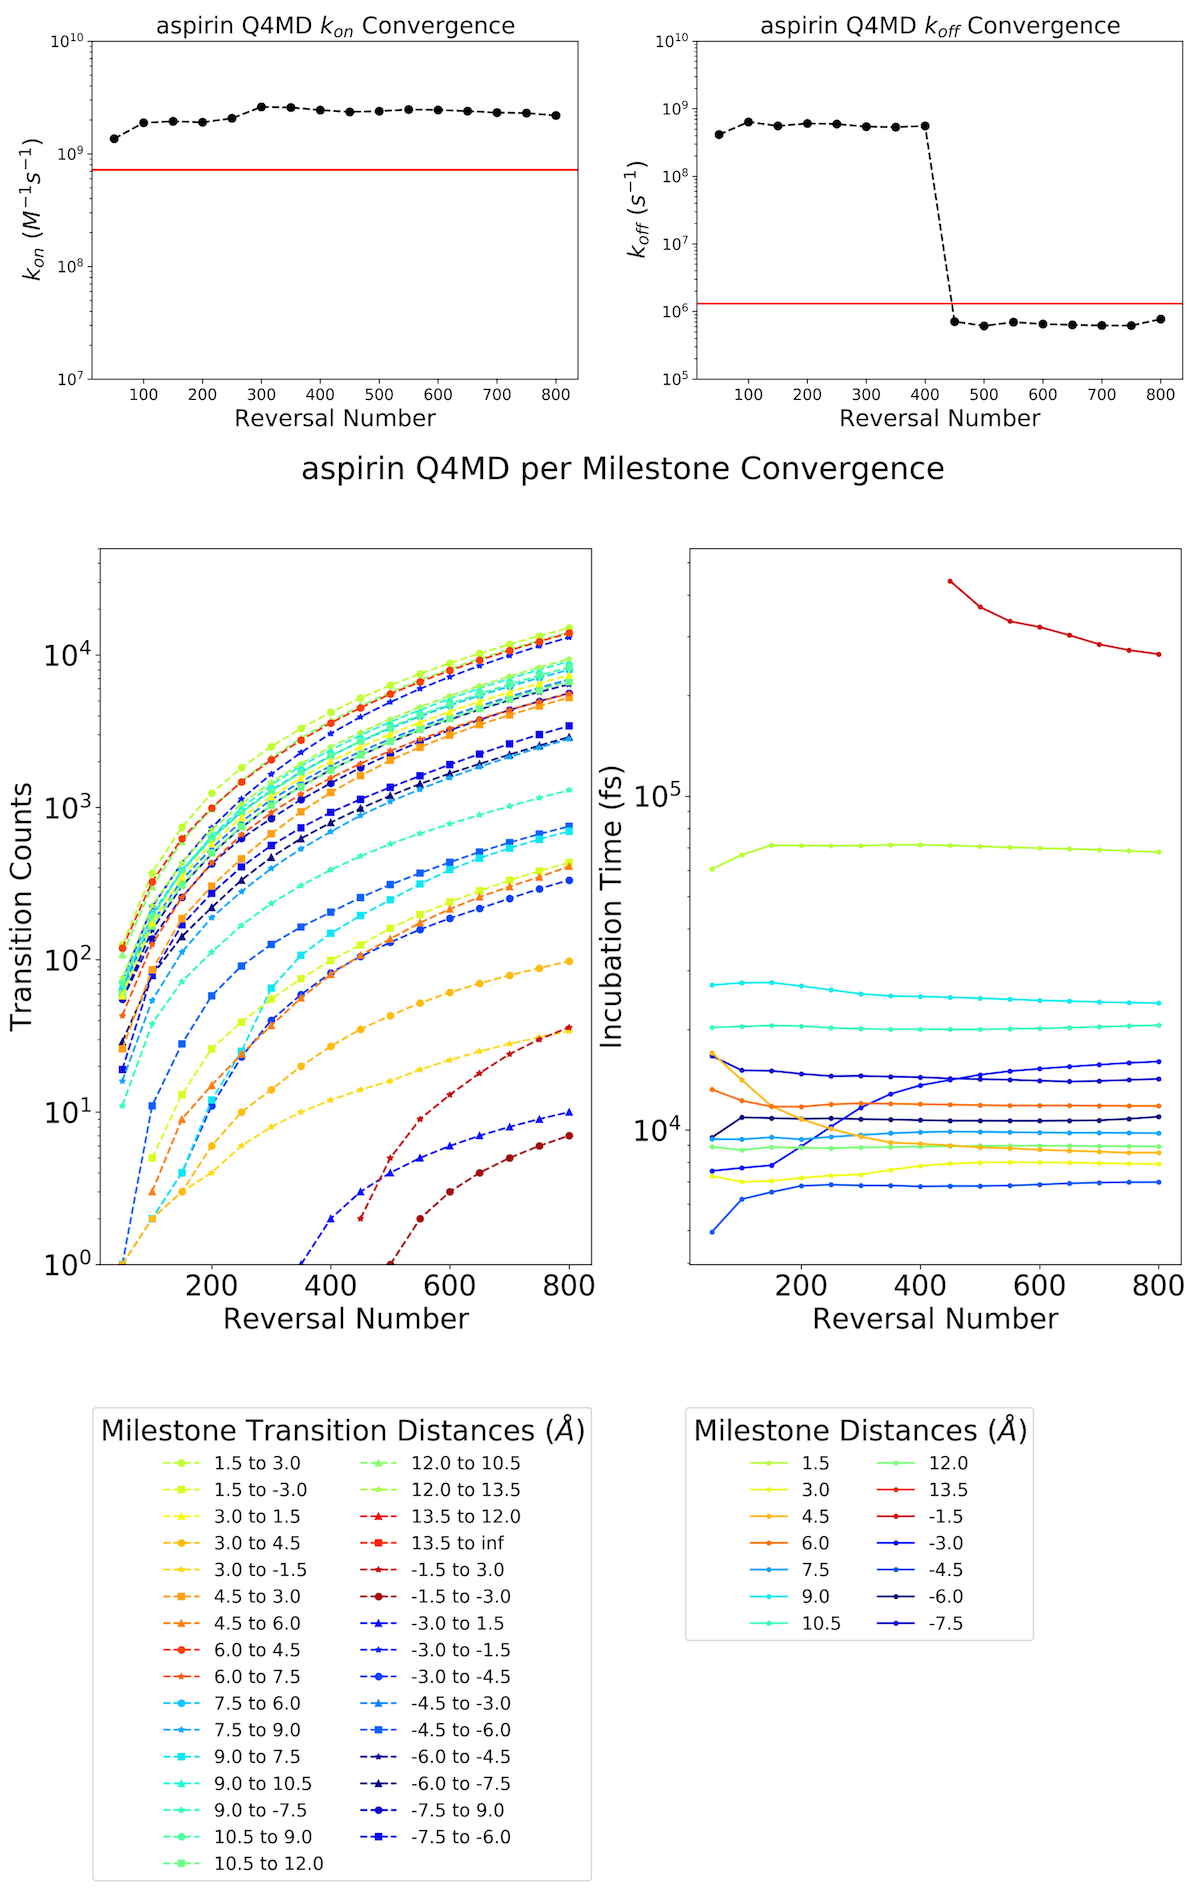
\includegraphics{../images/q4md_convergence_images/aspirin_q4md_complete.png}
    \caption{aspirin Q4MD per milestone convergence plot}
    \label{fig:aspirin_q4md_conv}
\end{figure}

\newpage 

\bibliography{../library.bib}

\end{document}

